\documentclass[thesismargins, thesislinespacing]{rnthesis}
\usepackage[slovak]{babel}
\usepackage[utf8]{inputenc}
\usepackage[]{graphicx}
\usepackage{nomencl}
\usepackage{lineno} 
\usepackage{caption}
\usepackage{subcaption}
\usepackage{braket}
\usepackage{multirow}

\title{}
\author{Lucia Anna Husová}
\typprace{Diplomová}
\rok{2018}
\miesto{Košice}
\odbor{Fyzika}
\podakovanie{
Na tomto mieste sa chcem poďakovať vedúcemu mojej práce doc. RNDr. Marekovi Bombarovi, PhD. za odborné rady a   osobný prístup.  Taktiež sa chcem poďakovať priateľovi Martinovi a rodičom za osobnú podporu.  	
  
} 
\veduci{doc. RNDr. Marek Bombara, PhD.}
\pracovisko{Ústav fyzikálnych vied, Katedra jadrovej a subjadrovej fyziky}

\abstract{
	
	The low energy jets are hardly identified in heavy ions collisions due to high background and the possible shape deformation. Therefore the two-particle correlation method is used to study these low energy jets in heavy ions collisions.\\
	In this thesis, the results of two-particle correlation method applied on the proton-proton collisions data at 13~TeV collected by the ALICE experiment at the LHC are presented. The yields for near-side and away-side peak for identified and unidentified trigger particles as a function of transversal momentum of trigger particles and multiplicity were measured. The structures of two-dimensional correlation function were also studied. The hadrons $K^0_S$, $\Lambda$ a $\bar{\Lambda}$ were chosen as identified trigger particles, due to their easy indentification at high transversal momentum, thanks to their decay topology.  

}


\abstrakt{
	
	Nízkoenergetické jety vzniknuté v zrážkach ťažkých iónov sú ťažko identifikovateľné vzhľadom na vysoké pozadie a možnú deformáciu ich tvaru, preto sa na ich štúdium, najmä v zrážkach ťažkých iónov, využíva metóda dvojčasticových korelácií.\\
	V tejto práci sú prezentované výsledky metódy dvojčasticových korelácií aplikovanej na dáta z protónovo-protónových zrážok pri energii 13 TeV zozbieraných na experimente ALICE na urýchľovači LHC. Merané boli výťažky pre priľahlý aj protiľahlý pík pre identifikované aj neidentifikované trigrovacie častice v závislosti od priečnej hybnosti trigrovacích častíc a multiplicity zrážok. Skúmané boli aj štruktúry dvojrozmerných korelačných funkcií v závislosti od multiplicity. Za identifikované trigrovacie častice boli zvolené podivné hadróny $K^0_S$, $\Lambda$ a $\bar{\Lambda}$, ktoré sa ľahko identifikujú aj pre vysoké priečne hybnosti vďaka svojej rozpadovej topológii.

\newpage
}

\makeglossary


\bibliographystyle{alpha}
%\linenumbers 
\begin{document}
\begin{center}
	{\Large Univerzita Pavla Jozefa Šafárika v Košiciach} \\
	%\end{center}
	%\begin{center}
	{\Large Prírodovedecká fakulta} 
\end{center}

\vspace*{2cm}

\begin{figure}[htbp!]
	\begin{center}
		
\includegraphics[width=3cm]{./Obrazky_praca/logo-pf-upjs-cb.jpg}
	\end{center}
\end{figure}

\vspace*{2cm}

\begin{center}
	%\vspace*{7cm}
	{\LARGE\bf Uhlové korelácie s podivnými časticami}
\end{center}

\begin{center}
	{\large Diplomová práca}
\end{center}

\vspace*{5cm}
\begin{flushleft}
{\bf Študijný odbor:}{ Jadrová a subjadrová fyzika} \\
{\bf Školiace pracovisko: }{Katedra jadrovej a subjadrovej fyziky}\\
{\bf Vedúci práce: }{doc. RNDr. Marek Bombara, PhD.}\\
\end{flushleft}
 
 \vspace*{2cm}
 \begin{flushleft}
{\large Košice 2018}
\hspace*{5cm}
{\large Bc. Lucia Anna Husová}
\end{flushleft}

\thispagestyle{empty}
\newpage

\maketitle
\newpage
\tableofcontents
\newpage

\chapter*{Zoznam skratiek a značiek}
\addcontentsline{toc}{chapter}{Zoznam skratiek a značiek}
\begin{itemize}
	\item[] LHC - Large Hadron Collider
	\item[] CERN - Conseil Européen pour la Recherche Nucléaire
	\item[] ŠM - Štandardný model
	\item[] QGP - Kvarkovo-gluónová plazma
	\item[] ALICE - A Large Ion Collider Experiment
	\item[] SLAC - Stanford Linear Accelerator Center
	\item[] QCD - Kvantová chromodynamika
	\item[] QED - Kvantová elektrodynamika
	\item[] LHCb - Large Hadron Collider beauty experiment
	\item[] GeV - gigaelektrónvolt
	\item[] c - rýchlosť svetla vo vákuu
	\item[] $m^3$ - meter kubický
	\item[] TeV - teraelektrónvolt
	\item[] $p_T$ - priečna hybnosť; $p_T=\sqrt{p_{x}^2+p_{y}^2}$
	\item[] $\phi$ - azimutálny uhol
	\item[] $\theta$ - polárny uhol
	\item[] $\eta$ - pseudorapidita; $\eta=-\ln \tan {\frac{\theta}{2}}$
	\item[] $\alpha_S$ - konštanta silnej interakcie
	\item[] SU(3) - špeciálna unitárna grupa matíc 3$\times$3
	\item[] $\sqrt{s_{NN}}$ - energia zrážky na jeden nukleónovo-nukleónový pár v ťažiskovej sústave 
	\item[] CGC - Color Glass Condensate
	\item[] fm - femtometer ($10^{-15}$m)
	\item[] SPS - Super Proton Synchrotron 
	\item[] RHIC - Relativistic Heavy Ion Collider
	\item[] STAR - Solenoidal Tracker at RHIC
	\item[] $V^{0}$ - neutrálna slabo sa rozpadávajúca častica, ktorej topológia rozpadu pripomína písmeno V
	\item[] TPC - Time Projection Chamber
	\item[] CMS - Compact Muon Solenoid
	\item[] T - tesla
	\item[] ITS - Inner Tracking System
	\item[] SPD - Silicon Pixel Detector
	 \item[] SDD - Silicon Drift Detector
	 \item[] SSD - Silicon Strip Detector
	 \item[] FMD - Forward Multiplicity Detector
	 \item[] kV - kilovolt
	 \item[] ESD - Event Summary Data
	 \item[] AOD - Analysis Object Data
	 \item[] MC - Monte Carlo
	 \item[] DCA - Distance of Closest Approach 
	 
\end{itemize}
\newpage


\chapter*{Úvod}
\addcontentsline{toc}{chapter}{Úvod}
Ani v súčasnej dobe nevieme nájsť odpovede na množstvo fundamentálnych otázok, preto si fyzika vysokých energií stále udržuje primát jednej z najaktívnejších oblastí fyziky. Na tento účel bol postavený najväčší urýchľovač častíc LHC (Large Hadron Collider) v laboratóriu CERN, ktorý nie je zameraný len na štúdium novej fyziky, ale aj na testovanie správnosti Štandardného modelu (ŠM) elementárnych častíc. Na LHC sa okrem protónovo-protónových zrážok skúmajú aj zrážky jadier olova, pri ktorých  sa vytvára kvarkovo-gluónová plazma (QGP), o ktorej sa predpokladá, že ňou bol tvorený Vesmír tesne po Veľkom tresku. 

Vlastnosti QGP sa vo väčšine prípadov skúmajú nepriamo prostredníctvom \-had\-ró\-nov, ktoré obsahujú kvarky a gluóny pochádzajúce z plazmy. Jedným z populárnych \-spô\-so\-bov sú tzv. "hard probes". Ide o rýchle partóny, ktoré interagujú s plazmou. Tie následne rozpoznávame v detektoroch ako spŕšky hadrónov (jety). Jety sa dajú skúmať \-pria\-mo alebo nepriamo, napr. metódou dvojčasticových korelácií. Jednou zo zaujímavých otázok v oblasti "hard probes" \-je, ako závisí interakcia rýchleho partónu s plazmou od farebného náboja. Partón môže niesť farbu (kvark), antifarbu (antikvark) alebo kombináciu oboch (gluón). Keďže kvarkové a gluónové jety majú rôzne vlastnosti a v~priemere pozostávajú z rôznych hadrónov, táto problematika by sa mohla dať študovať pomocou korelácií s identifikovanými časticami.  

\chapter{Kvantová chromodynamika}

Po objave vnútornej štruktúry protónov v 60-tych rokoch minulého storočia v laboratóriu SLAC (Stanford Linear Accelerator Center) bolo potrebné vytvoriť teoretický model popisujúci správanie sa novoobjavených častíc - partónov, ktoré boli neskôr priradené k teoreticky predpovedaným kvarkom a gluónom. Na pochopenie interakcie medzi partónmi vznikla kvantová chromodynamika (QCD), ktorá bola sformulovaná na základe symetrií, podobne ako staršia kvantová elekrodynamika (QED). V QED je zdrojom vzájomného pôsobenia elektrický náboj. Jeho analógiou v QCD je farebný náboj ako zdroj silnej interakcie, ktorý môže nadobúdať šesť stavov (modrý, červený, zelený, antimodrý, antičervený, antizelený) \footnote{druhy farebného náboja nesúvisia s farbami viditeľnej časti elektromagnetického spektra}.

\section{Farebný náboj}
Farba, ako nové kvantové číslo, bola zavedená kvôli Pauliho vylučovaciemu princípu, ktorý hovorí, že fermióny (častice s polčíselným spinom) v jednom kvantovo-me\-cha\-nic\-kom systéme nemôžu mať všetky kvantové čísla rovnaké. Vedelo sa však o existencii častíc, ktoré sa skladajú z kvarkov s rovnakými dovtedy známymi kvantovými číslami (napr. $\Delta^{++}$ (uuu) alebo $\Omega^{-}$ (sss)). Ponúkalo sa niekoľko vysvetlení:
\begin{itemize}
	\item Neplatí Pauliho vylučovací princíp.
	\item Kvarky nie sú fermióny, ale bozóny s celočíselným spinom.
	\item Existuje ďalšie kvantové číslo.
\end{itemize}
Keďže Pauliho princíp je založený na kauzalite, nemožno o ňom prehlásiť, že je neplatný. Preto sa najpriateľnejšou možnosťou ukázalo zavedenie nového kvantového čísla, farby. Vlnová funkcia kvantovo-mechanického systému sa stáva opäť antisymetrickou a tým pádom zostáva platný Pauliho vylučovací princíp:
\begin{equation}
	\Psi_{TOTAL}=\Psi_{SPACE}*\Psi_{SPIN}*\Psi_{FLAVOUR}*\Psi_{COLOUR}, 
\end{equation}   
kde $\Psi_{SPACE}$ je priestorová časť vlnovej funkcie, $\Psi_{SPIN}$ je spinová časť, $\Psi_{FLAVOUR}$ je časť popisujúca druh kvarku a $\Psi_{COLOUR}$ je časť určujúca farebný náboj~\cite{1}.

Pri zohľadnení farebného náboja sa vyriešili aj iné dovtedy nepochopené rozdiely medzi výpočtami a výsledkami experimentov, ako napríklad účinný prierez elektromagnetického rozpadu $\pi^0$ mezónu na dva fotóny alebo $\tau$ leptónu na hadróny. 

Farebný náboj však nenesú len samotné kvarky, ale aj nosiče silnej interakcie - gluóny, ktoré sú dvojfarebné (sú nosičom farby a antifarby). Preto môžu interagovať ako s kvarkami, tak aj so sebou navzájom. Predpokladá sa, že jedným z dôsledkov tejto vlastnosti je, že farebné častice nemôžu existovať ako voľné častice, a teda farebný náboj je uväznený vnútri hadrónov.

Samointerakcia gluónov vyplýva aj z vlastností špeciálnej unitárnej grupy SU(3), ktorá popisuje transformácie v rámci QCD. Keďže táto grupa nie je Abelovská, jednotlivé transformácie spolu nekomutujú a teda v Lagrangiáne popisujúcom silnú interakciu vznikajú samointerakčné členy gluónov (interakcia 3 alebo 4 gluónov). Grupa SU(3) má 8 voľných parametrov, preto sa vyžaduje existencia 8 rôznych gluónov. Gluóny môžu vrámci tejto grupy tvoriť oktet alebo singlet. Singlet však nie je pozorovaný. Jeho existencia by viedla ku vzniku ďaleko-dosahovej silnej interakcie a vlastnosťami by sa podobal na fotón. 

Z experimentov sa zistilo, že v prírode existujú iba navonok bezfarebné multiplety kvarkov tvoriace hadróny, a teda všetky z nich sú singlety (nemenia farebný náboj počas interakcie). Sú to:
\begin{itemize}
	\item mezóny - kombinácia farby a antifarby ($q \bar q$)
	\item "biele" baryóny - kombinácia troch rôznych farieb ($qqq$) a antibaryóny - kombinácia troch rôznych antifarieb ($\bar q \bar q \bar q$)
	\item exotické stavy - tetrakvarky ($q \bar q q \bar q$), pozorované v apríli 2014 \cite{tetra} a pentakvarky ($qqqq \bar q $), pozorované v júli 2015 na experimente LHCb \cite{2}
\end{itemize}

\section{Asymptotická sloboda}
Ďalšia vlastnosť QCD, ktorá je dôsledkom samointerakcie medzi gluónmi, je asymptotická sloboda. 
Veľkosť náboja v silnej, ale aj v elekromagnetickej interakcii závisí od vzdialenosti, z ktorej náboj študujeme. Pri štúdiu elektromagnetickej interakcie na veľmi malých vzdialenostiach nemožno zanedbávať kvantovo-mechanické efekty, ako je napr. polarizácia vákua. V okolí elektrónu sa vytvoria virtuálne páry elektrónov a pozitrónov a kvôli ich  orientácii vznikne v okolí pôvodného elektrónu oblak kladného náboja. Z tohto dôvodu pri väčších vzdialenostiach nameriame tzv. "renormalizovaný" \-e\-lektrický náboj, ktorý má menšiu hodnotu ako pôvodný netienený náboj.

Podobný proces nastáva aj pri silnej interakcii. V okolí farebne nabitého kvarku sa vytvárajú páry kvark-antikvark a gluóny. Na rozdiel od elektromagnetickej interakcie, kde fotóny na seba navzájom nepôsobia, gluóny na seba pri silnej interakcii pôsobia. To vedie k tomu, že sila silnej interakcie sa so zväčšujúcou vzdialenosťou zväčšuje. Na malých vzdialenostiach môžeme povedať, že silná interakcia asymptoticky zaniká (asymptotická sloboda), aj keď je stále väčšia ako elektromagnetická, a z kvarkov a gluónov sa z pohľadu silnej interakcie stávajú voľné častice. 

Táto vlastnosť sa tiež prejavuje pri vysokoenergetických nepružných zrážkach. Čím majú zrážajúce sa častice vyššiu hybnosť, tým je silná interakcia pôsobiaca medzi nimi slabšia (obr.~\ref{alfa}).
\begin{figure}
	\centering
	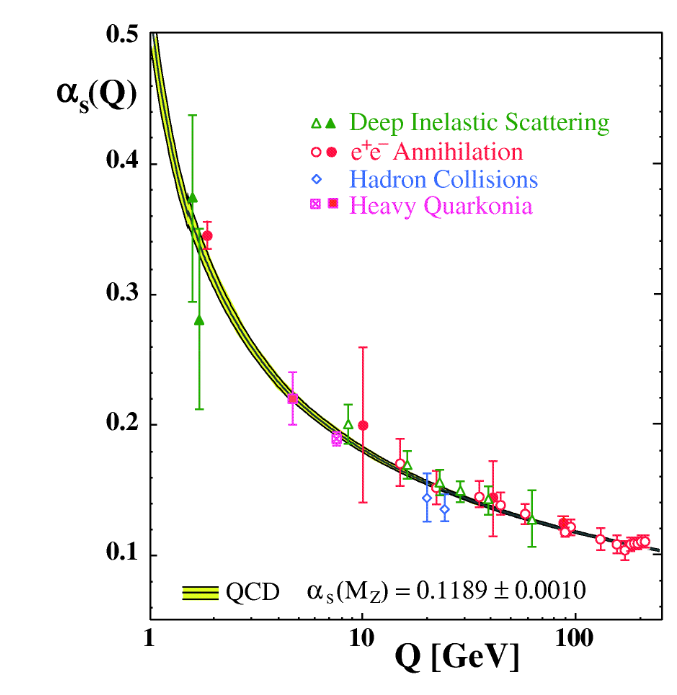
\includegraphics[scale=0.4]{./Obrazky_praca/zrazka.png}
	\caption{Závislosť konštanty silnej interakcie $\alpha_s$ od energetickej škály jednotlivých procesov Q \cite{3}}
	\label{alfa}
\end{figure}




\section{Jety}

Kvarky a gluóny sú uväznené vnútri hadrónov\footnote{Uväznenie kvarkov v hadrónoch je experimenálny fakt, ale na rozdiel od asymptotickej slobody zatiaľ nie je vysvetlené v QCD.}, a teda nemôžeme pozorovať vlastnosti kvarkov a gluónov priamo. Pri udelení dostatočnej energie partónu v hadróne sa táto energia premení na spŕšku hadrónov v jednom smere (tzv. jet), v ktorej sa nachádza hadrón obsahujúci pôvodný partón. V experimentoch je jet definovaný ako skupina energe\-tických hadrónov pohybujúcich sa v jednom smere, ktoré je možné ohraničiť mysleným kužeľom so stredom určeným smerom pohybu originálneho partónu (tzv. jet axis) a s polomerom R~\cite{4}:
\begin{equation}
\sqrt{\Delta \phi^2 + \Delta \eta^2}<R=1,
\end{equation}
kde $\Delta \phi$ je rozdiel azimutálnych uhlov hadrónu v jete a pôvodného partónu, $\Delta \eta$ je rozdiel pseudorapidít\footnote{Pseudorapidita $\eta$ je funkciou polárneho uhla $\theta$: $\eta = - \ln( \tan (\frac{\theta}{2}))$.} hadrónu v jete a pôvodného partónu.

\subsection{Lundský strunový model}
Kým interakcie partónov pri vysokých energiách sú dobre popísané pomocou QCD, na popis vytvárania hadrónov v jetoch si musíme pomôcť fenomenologickými \-mo\-del\-mi. Jeden zo základných modelov, ktorý je prítomný vo väčšine Monte Carlo (MC) generátorov vo fyzike vysokých energií, je Lundský strunový model.

Pre potenciál viazaného stavu kvarku a antikvarku platí:
\begin{equation}
	V(r) \approx - \frac{4}{3} \frac{\alpha_s}{r} + \kappa r \approx - \frac{0.13}{r} + r~\cite{5}
\end{equation}

Na veľmi malých vzdialenostiach ($r\rightarrow0$) prevláda potenciál Coulombovského poľa (obr.~\ref{elpole}). Pri vzájomnom vzďaľovaní sa kvarkov začne prevládať lineárna časť potenciálu a na rozdiel od elekromagnetického poľa sa kvôli samointerakcii gluónov budú siločiary k sebe približovať a vytvoria tvar podobný trubici (obr.~\ref{chrompole}).

Ak je vzdialenosť medzi dvoma kvarkami dostačujúca, z energie poľa sa vytvorí nový pár častíc kvark-antikvark (obr.~\ref{jet}). Takto to pokračuje ďalej, pokiaľ majú vzďaľujúce sa partóny dostatok energie na vytvorenie nového páru kvark-antikvark. Celý proces pripomína trhanie struny, odkiaľ pochádza aj názov modelu.

\begin{figure}[hbtp!]
	\centering
	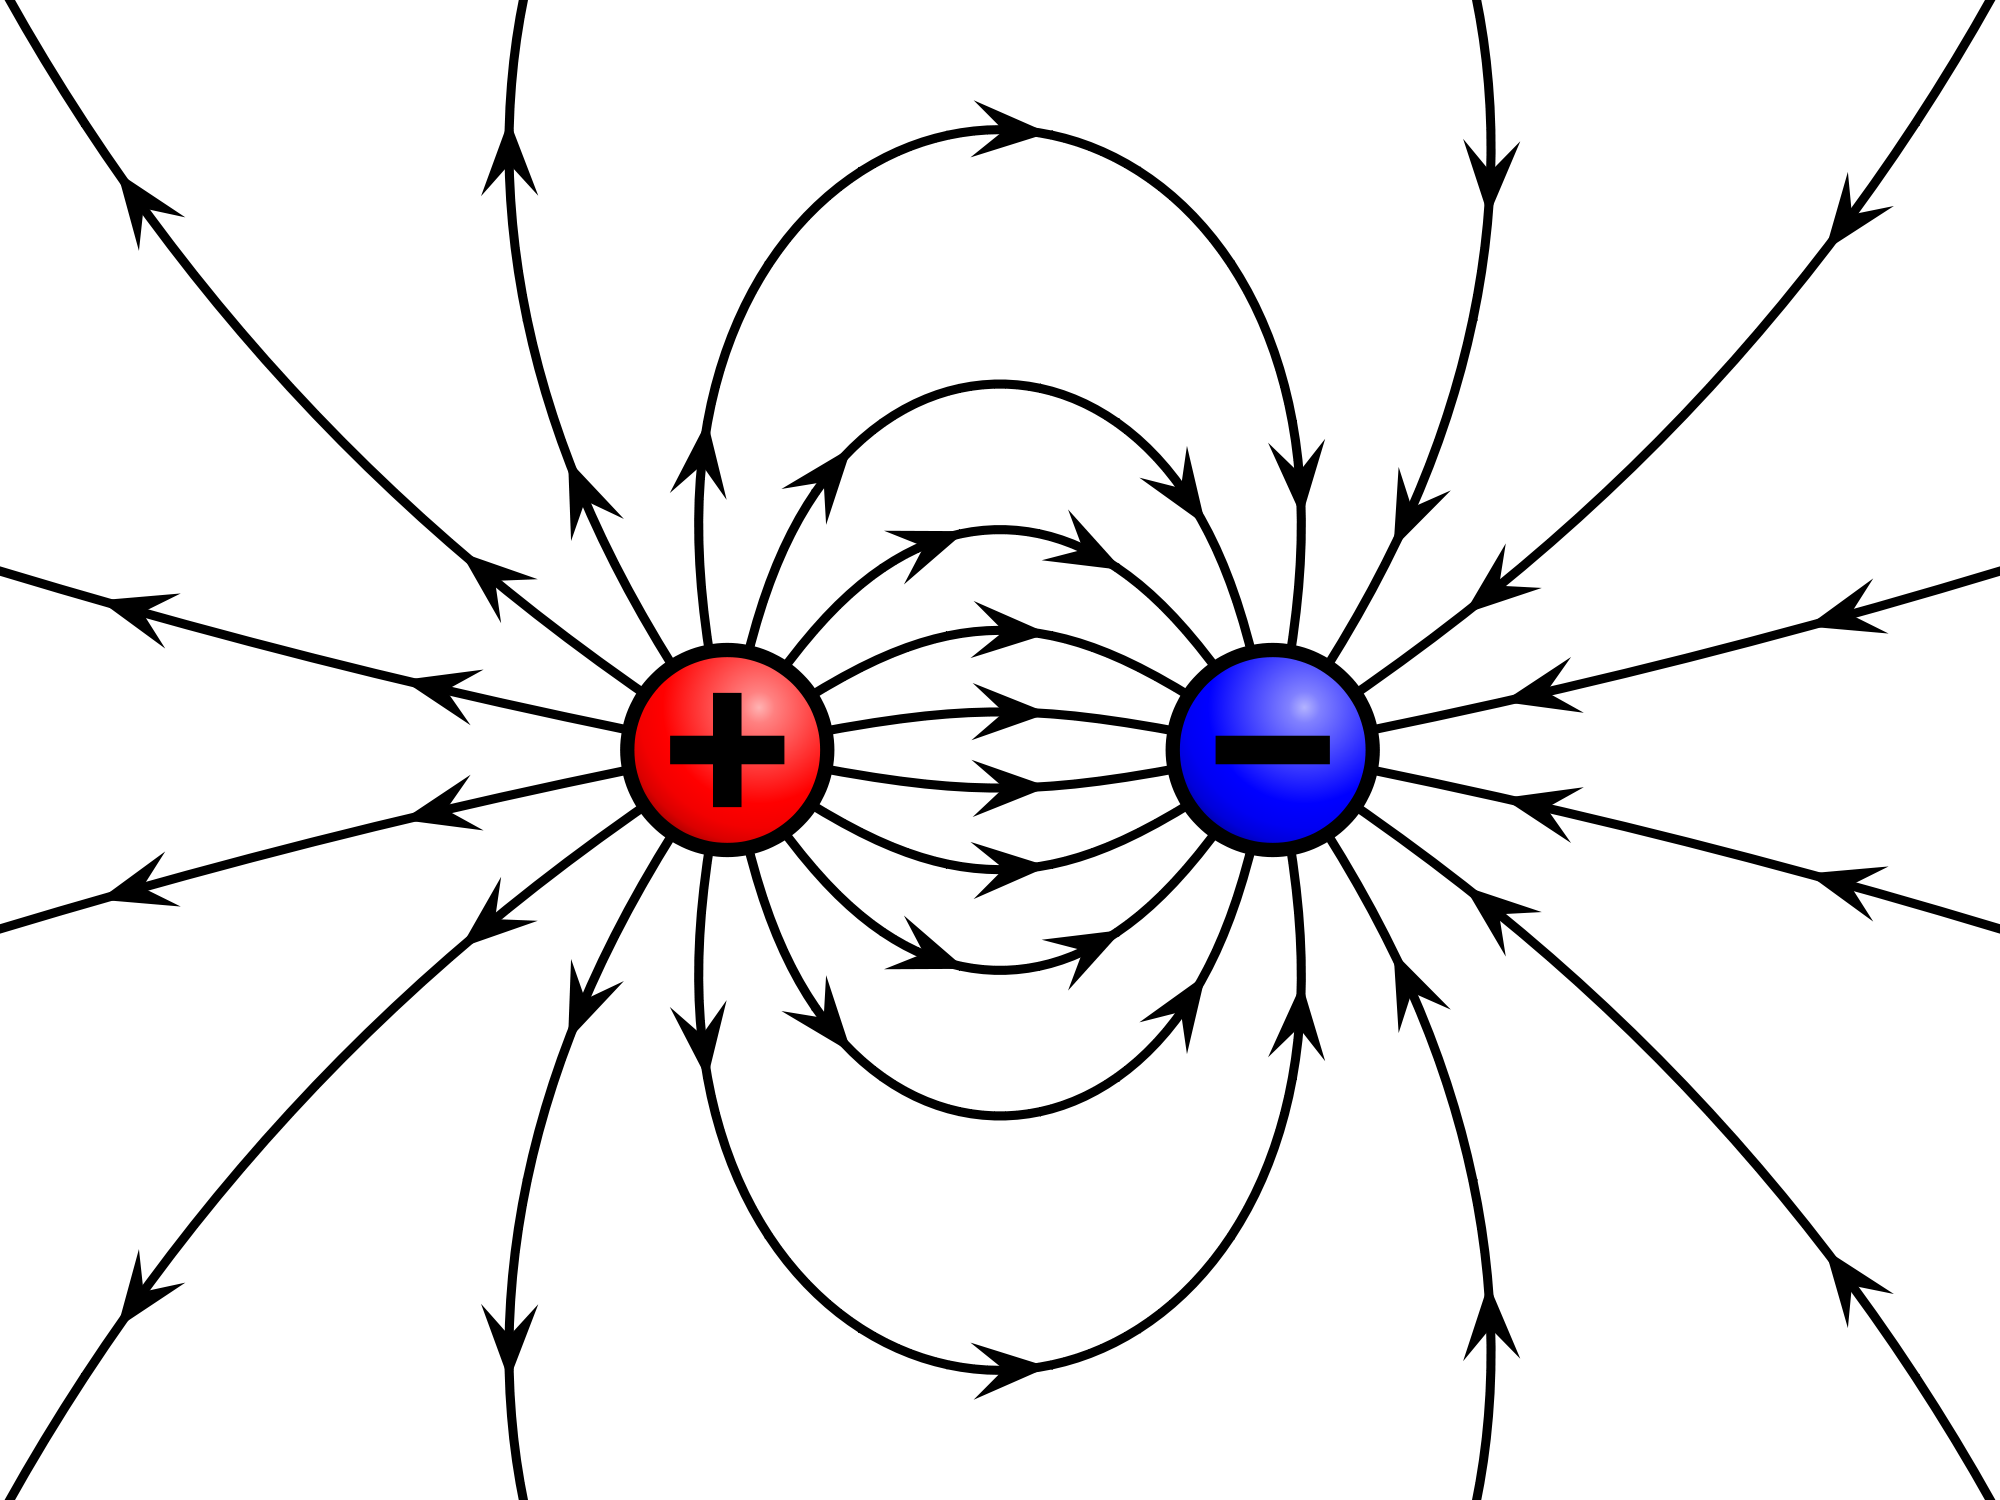
\includegraphics[scale=0.08]{./Obrazky_praca/el_pole.png}
	\caption{Siločiary elektrického poľa sa od seba so zväčšujúcou sa vzdialenosťou vzďaľujú~\cite{6}.}
	\label{elpole}
\end{figure}
\begin{figure}[hbtp!]
	\centering
	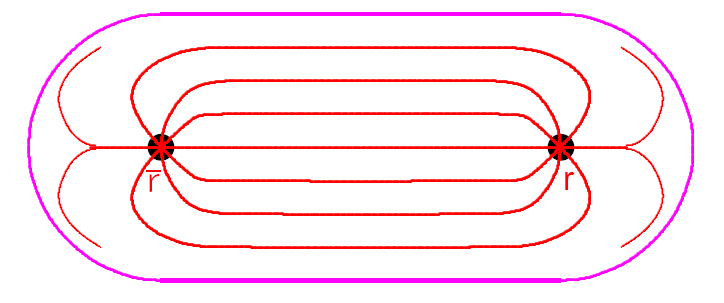
\includegraphics[scale=0.25]{./Obrazky_praca/chromo_pole.png}
	\caption {Siločiary chromodynamického poľa sa k sebe so zväčšujúcou sa vzdialenosťou približujú~\cite{7}.}
	\label{chrompole}
\end{figure}

\begin{figure}[hbtp!]
	\begin{center}
	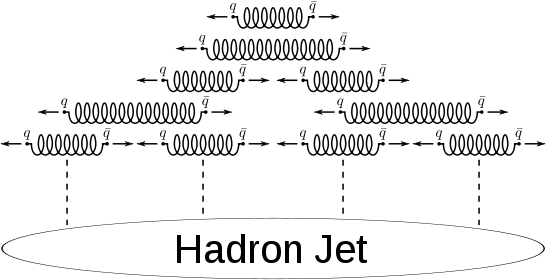
\includegraphics[scale=0.5]{./Obrazky_praca/jet.png}
	\caption{Tvorba jetu pripomína trhanie struny. Čím viac od seba naťahujeme konce struny, tým väčšiu silu musíme vynaložiť. Pri prasknutí struny získame dve nové struny~\cite{8}.}
	\label{jet}
	\end{center}
\end{figure}  

\subsection{Kvarkové a gluónové jety}
\label{kvgl}
Výsledky experimentov ukazujú, že vlastnosti jetov sa líšia podľa toho, z akého partónu jet vznikol. Kvarkové a gluónové jety sa líšia v multiplicite~\cite{{10}}, šírke jetu a v produkcii finálnych mezónov a baryónov~\cite{clanokqg}. Jety, ktoré vznikli z gluónov, majú vo všeobecnosti väčšiu multiplicitu (obr.~\ref{multiplic}), sú širšie a vytvára sa väčšie množstvo baryónov ako v kvarkových, pričom produkcia mezónov je približne rovnaká. V analýze~\cite{clanokqg} konkrétne namerali o 40\% viac $\Lambda$ baryónov v gluónových jetoch, pričom počet $K^{0}_{S}$ mezónov bol prižne rovanký v oboch druhoch jetov. Jednou z metód, pomocou ktorých by sme mohli odlíšiť kvarkové jety od gluónových, je metóda dvojčasticových korelácií s identifikovanou trigrovacou časticou(viac v sekcii \ref{korel}).  

\begin{figure}[hbtp!]
	\begin{center}
		\includegraphics[width=0.8\textwidth]{./Obrazky_praca/multiplic.png}
		\caption{Porovnanie priemernej multiplicity nabitých hadrónov v kvarkových a gluónových jetoch v rôznych experimentoch v závislosti od energie~\cite{10}.}
		\label{multiplic}
	\end{center}
\end{figure}  

\section{Kvarkovo-gluónová plazma}

Pri extrémnych podmienkach (vysoká teplota, vysoká hustota) sa môžu kvarky a~gluó\-ny zbaviť svojho uväznenia v hadrónoch. Keďže tieto partóny sa môžu pohybovať voľne v rámci určitého objemu, nazýva sa takýto stav hmoty aj kvarkovo-gluónová plazma (QGP). Predpokladá sa, že tesne po Veľkom tresku bola teplota dostatočne vysoká, aby bol celý Vesmír tvorený QGP. V súčasnosti by sa QGP mohla nachádzať v jadrách niektorých neutrónových hviezd, kde by mala byť dostatočná hustota na to, aby sa kvarky a gluóny uvoľnili z neutrónov.

\begin{figure}[hbtp!]
	\begin{center}
		\includegraphics[scale=0.5]{./Obrazky_praca/phasDiag.png}
		\caption{ Fázový diagram QGP \cite{phasDiagram}}
		\label{fazDiag}
	\end{center}
\end{figure}  

QGP vzniká pri vysokých teplotách a/alebo pri vysokom baryónovom potenciáli ako je vidieť na fázovom diagrame na obr.~\ref{fazDiag}. QGP je preto možné vytvoriť aj laboratórnych podmienkach pri zrážkach ťažkých iónov, v súčastnosti napríklad na urýchľovačoch RHIC a LHC. Pri energiách dosahovaných na týchto urýchľovačoch sú zrážajúce sa jadrá Lorentzovsky deformované do formy plochých diskov a hustota morských partónov\footnote{Pri vysokých enrgiách sú pozorované aj kvantovo mechanické fluktuácie vnútri protónov. Vplyvom fluktuácií sa gluóny zmenia na pár kvark antikvark a tie späť anihilujú na gluóny.} sa zvyšuje. Tento stav hmoty sa nazýva CGC\footnote{z angl. Colour Glass Condesate - univerzálna forma hmoty tvoriaca vysokoenergetické hadróny\cite{hevion}. Napríklad protón pri LHC energiách je tvorený touto hmotou.}. V takejto forme hmoty je vysoká hustota energie gluónov a ich vzájomné interakcie sa stávajú dôležitejšími ako interakcie kvarkov. Tieto gluóny postupne termalizujú a vytvárajú QGP. Prechod medzi CGC a QGP má ešte jeden medzistav nazývaný glasma\footnote{Hustá hmota interpolujúca prechod od CGC a QGP, ktorá sa ale svojimi vlastnosťami líši od oboch týchto stavov\cite{hevion}. Jedná sa o plazmu tvorenú gluónmi.}\cite{glasma}.

Keďže ióny sa zrážajú s vysokou energiou, v mieste zrážky sa nachádza vysoká hustota energie a vytvorí sa tlakový gradient, vďaka ktorému hmota prudko expanduje. Tento proces sa niekedy v odbornej literatúre označuje ako “Little Bang”. Za veľmi krátky čas ($\tau_{form}<1$ fm/c)  sa novovytvorené kvarky a gluóny dostanú do termodynamickej rovnováhy a vytvoria kvapku QGP, ktorej vlastnosti sa podobajú na vlastnosti ideálnej kvapaliny. Na popis časovo-priestorového vývoja QGP je Lagrangian QCD príliš zložitý, a preto sa používajú hydrodynamické modely založené na lokálnej termodynamickej rovnováhe (stavové rovnice a relativistická hydrodynamika).

Systém bez vonkajšieho tlaku rýchlo expanduje a chladne a po čase $\approx 10$ fm/c a pri kritickej teplote 180~MeV\footnote{Vo fyzike elementárnych častíc sa na určenie teploty používajú jednotky eV, kde $\frac{1eV}{k}= 11605K$, a teda 180MeV zodpovedá teplote $2.1\times10^{12}K$.}, ktorá je blízko teplote fázového prechodu, sa partóny formujú do hadrónov. Vytvorí sa zmiešaný stav QGP a hadrónového plynu, ktorý chladne a expanduje.  Pri teplote 176 MeV\cite{tempr} nastáva tzv. chemický "freeze-out\-", t.j. počet jednotlivých druhov hadrónov sa ustáli a vytvorí sa čistý hadrónový plyn, kde hadróny už môžu interagovať iba pružne. Úplne interagovať prestávajú pri teplote 89 až 127 MeV v závislosti od centrality zrážky\cite{kinfrezze}, kedy nastáva kinematický "freeze-out"\footnote{Vzdialenosti medzi časticami sú väčšie ako ich stredné voľné dráhy. } \-a hadróny sa rozletia do detektorov (obr.~\ref{QGP}) . Keďže QGP existuje veľmi krátky čas, jej vlastnosti je možné skúmať iba nepriamo pomocou hadrónov\footnote{Výnimkou sú napr. fotóny vznikajúce priamo v plazme, keďže ich stredná voľná dráha je väčšia ako rozmery QGP vzniknutej pri zrážke dvoch jadier.}.  

\begin{figure}[hbtp!]
	\begin{center}
		\includegraphics[scale=0.35]{./Obrazky_praca/QGP1.png}
		\caption{ Časový a priestorový vývoj QGP \cite{vyvoj}}
		\label{QGP}
	\end{center}
\end{figure}  

Pomocou QGP možno skúmať priamu interakciu častíc s  farebným nábojom, pretože je tvorená voľnými partónmi nesúcimi farebný naboj, ktorý je inak uväznený v hadrónoch, a overovať tak predpovede QCD. 

\subsection{Signatúry kvarkovo-gluónovej plazmy} 

Prítomnosť QGP pri zrážkach relativistických ťažkých iónov je indikovaná rôznymi znakmi, ktoré závisia najmä od energie zrážky. Preto boli na jednotlivých urýchľovačoch pozorované iné prejavy QGP\footnote{Výber jednotlivých signatúr je subjektívny. Snaha bola vybrať tie najzaujímavejšie, keďže ich je niekoľko desiatok.}:
\begin{itemize}
	\item \textbf{SPS}
	\begin{itemize}
		\item "rozpustenie" (z angl. melting) kvarkonie\footnote{Mezón tvorený kvarkom a antikvarkom toho istého druhu, napr. $J/ \psi$ tvorený párom $c \bar{c}$ } - interakcia medzi kvarkom a antikvarkom v mezóne je tienená ostatnými kvarkami a gluónmi v QGP a kvarkonium sa “rozpustí". Tento jav už pri vyšších energiách nie je taký výrazný, pretože v zrážke vznikne viac kvarkonie, ktorá sa následne rozpúšťa v QGP. Preto je vyššia pravdepodobnosť, že 2 kvarky z pôvodne rôznych častíc sa v QGP spoja a vytvoria dodatočnú kvarkoniu \cite{JpsiSupp}.
		\item zvýšená produkcia podivnosti oproti protónovo-protónovým zrážkam. Tvorba podivnosti z termálnych gluónov bola predpovedaná ako jedna zo \-zák\-lad\-ných charakteristík QGP. Pár $s \bar{s}$ vzniká na jednom mieste a v jednom čase v QGP, ale podivné hadróny sú pozorované akoby vznikali na opačných koncoch QGP štatisticky nezávisle na sebe. Fázový priestor  teda nie je obmedzený ako v protónovo-protónových zrážkach.
		Čím sú hadróny viac podivnejšie (obsahujú väčší podiel podivných kvarkov resp. antikvarkov), tým je zvýšená produkcia viditeľnejšia. To bolo namerané na experimente WA97 na urýchľovači SPS v CERNe \cite{zvysenie} (obr.~\ref{zvysenie}).
	\end{itemize}
	\item \textbf{RHIC}
	\begin{itemize}
		\item zhášanie jetov - jety pri prechode QGP strácajú energiu vplyvom pružných zrážok alebo radiačných procesov (gluon Bremsstrahlung)~\cite{rhic}.
		\item eliptický tok - pri jadrovo-jadrových zrážkach, ktoré nie sú úplne centrálne, sa QGP nevytvára vo forme gule ale v tvare pripomínajúcom mandľu (obr.\ref{elflow}). Tento tvar je zodpovedý za asymetriu v toku v smere interakčnej roviny\footnote{Rovina tvorená smerom zväzku a inpakt paramentrom, čo je nejkratšia vzdialenosť medzi stredmi zrážajúcich sa jadier.} a v smere kolmom na ňu \cite{elflow}. 
	\end{itemize}
	\item \textbf{LHC}
	\begin{itemize}
		\item v podstate všetky signatúry pozorované pri nižších energiách na urýchľovačoch SPS a RHIC
		\item pokles jadrového modifikačného faktora\footnote{Pomer počtu istého druhu častíc v zrážkach olovo-olovo ku preškálovanému počtu týchto častíc v protónovo-protónových zrážkach.} v závislosti od hmotnosti kvarku - v experimente bolo pozorované rôzne potlačenie B mezónov (b kvark), D mezónov (c kvark) a piónov (ľahké kvarky), pričom závislosť potlačania bola $R_{AA}(\pi)\approx R_{AA} (D)<R_{AA}(B)$\footnote{Čím väčšia hodnota pomeru $R_{AA}$, tým menšie potlačenie.} \cite{RAA}. Kvalitatívne to súhlasí s predpokladom, že energetické straty partónu v plazme sú nepriamoúmerné hmotnosti tohto partónu. 
		
	\end{itemize}
\end{itemize}

\begin{figure}[hbtp!]
	\begin{center}
		\includegraphics[scale=0.4]{./Obrazky_praca/zvysenie.png}
		\caption{ Zvýšenie výťažkov podivných hadrónov v jadrovo-jadrových zrážkach ako funkcia ich celkovej podivnosti \cite{zvysenie}}
		\label{zvysenie}
	\end{center}
\end{figure}  

\begin{figure}[hbtp!]
	\begin{center}
		\includegraphics[scale=0.35]{./Obrazky_praca/elipticflow.png}
		\caption{ Príklad "mandľovo tvarovanej" necentrálnej zrážky dvoch jadier \cite{elflow}.}
		\label{elflow}
	\end{center}
\end{figure}  

\subsection{Kvarkovo-gluónová plazma v zrážkach protón-protón?}
Prítomnosť QGP v jadrovo-jadrových zrážkach je akceptovaným a potvrdeným faktom. Nové merania protónovo-protónových a protónovo-olovených zrážok pri energiách na LHC odhalili pozorovanie niektorých znakov QGP aj v týchto malých systémoch. Jedným z nich je zvýšená produkcia podivnosti v pp a p-Pb zrážkach s vysokou multiplicitou\footnote{Multiplicita je stredná hodnota hustoty primárnych nabitých častíc v strednej rapidite   \newline  ($\braket{dN_{ch}/d\eta}_{|\eta|<0.5}$).}. Merané boli pomery výťažkov podivných hadrónov ku výťažkom piónov normovaných na ten istý pomer nezávislý na multiplicite v závislosti od multiplicity zrážky. Ako je vidieť na obr.\ref{strange}, pomer pre jednotlivé podivné a  multipodivné hadróny lineárne narastá so zväčšujúcou sa multiplicitou zrážok. Zvýšenia pre jednotlivé hadróny narastajú s ich podivnosťou, nie s ich hmotnosťou alebo baryónovým číslom. Tento jav je typický pre jadrovo-jadrové zrážky a je spájaný s výskytom QGP v týchto zrážkach \cite{nature}.  Ďalším znakom bol kolektívny tok pozorovaný v dvojčasticových koreláciách (viac v \ref{textAliceCms}).
\begin{figure}[hbtp!]
	\begin{center}
		\includegraphics[scale=0.6]{./Obrazky_praca/nature.png}
		\caption{ Pomery výťažkov podivných hadrónov ku piónom \cite{nature}.}
		\label{strange}
	\end{center}
\end{figure} 

\chapter{Dvojhadrónové korelácie na urýchľovačoch RHIC a LHC}

\section{Metóda dvojčasticových korelácii}
\label{korel}
Metóda dvojčasticových (dihadrónových) korelácii je jednou z nepriamych metód na štúdium jetov. Využíva sa najmä v jadrovo-jadrových zrážkach, kde kvôli \-mo\-di\-fi\-ká\-cii jetov vplyvom QGP nemožno použiť priame metódy, ktoré sú používané pri protónovo-protónových zrážkach.

Spočíva v zvolení intervalu priečnej hybnosti\footnote{Priečna hybnosť je definovaná ako: $p_T=\sqrt{p_x^2+p_y^2}$, pričom rovina $xy$ je kolmá na os zväzku v experimente.}, v ktorom sa hľadá častica s vysokou priečnou hybnosťou, tzv. trigrovacia častica ("trigger particle"), o ktorej sa predpokladá, že je to hadrón obsahujúci pôvodný partón. Tiež je potrebné zvoliť interval nižších hybností pre asociované častice ("\-associated particles"). Následne sa robia rozdiely v \-a\-zi\-mu\-tál\-nom uhle $\phi$ a pseudorapidite $\eta$ pre rôzne intervaly priečnej hybnosti trigrovacích a asociovaných častíc:

\begin{equation}
\Delta \phi = \phi_{trig} - \phi_{asoc}
\end{equation}

\begin{equation}
\Delta \eta = \eta_{trig} - \eta_{asoc}
\end{equation}

Tieto rozdiely sa plnia do dvojrozmerných histogramov, z ktorých sa robia projekcie na jednotlivé osi. V projekcii na $\Delta \phi$ sa vytvoria dva píky zodpovedajúce dvom jetom. Keďže pred zrážkou bola celková priečna hybnosť nulová, vytvorenie jedného jetu je sprevádzané vytvorením jetu na protiľahlej strane v rovine $xy$. Pík  so stredom v 0 sa nazýva priľahlý pík (v angličtine "near-side peak") a je spôsobený pármi, kde asociované častice pochádzajú z toho istého jetu ako trigrovacia častica. Druhý pík sa nachádza v okolí $\pi$ a je spôsobený takými pármi častíc, kde asociovaná častica pochádza z jetu, ktorý je oproti jetu, z ktorého je trigrovacia častica. Preto sa nazýva protiľahlý pík (v angličtine ''away-side peak'')(obr.~\ref{kor}). Iná situácia nastáva v pozdĺžnom smere. Partóny v protónoch vo zväzku môžu mať v princípe rôznu pozdĺžnu hybnosť, a teda, ak vidíme v detektore jet v pozdĺžnom smere, druhý nemusí byť na protiľahlej strane. Výberom trigrovacej častice vyberáme jety, ktoré sa nachádzajú v detektore a ich náprotivky sa nemusia nachádzať v skúmanom intervale $\Delta \eta$.

\begin{figure}[hbtp!]
	\begin{center}
		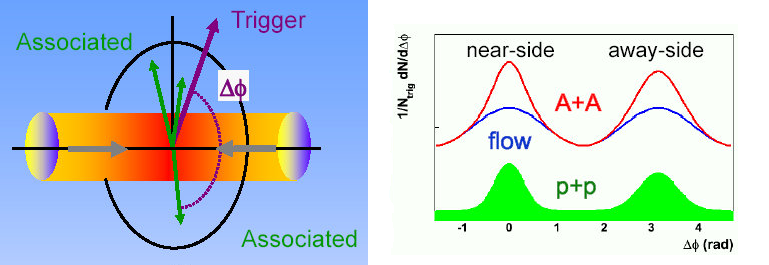
\includegraphics[width=\textwidth]{./Obrazky_praca/dijetcorrelations.png}
		\caption{Vľavo: Schéma polohy trigrovacej a asociovanej častice. Vpravo: Poloha priľahlého a protiľahlého píku pre protónovo-protónové a jadrovo-jadrové zrážky. Pozadie v protónovo-protónových zrážkach je konštantné, v jadrovo-jadrových zrážkach je \-mo\-di\-fi\-ko\-va\-né kolektívnym tokom (flow).}
		\label{kor}
	\end{center}
\end{figure}

Po korekciách na účinnosť rekonštrukcie dráh asociovaných častíc, po normovaní na počet trigrovacích častíc a po odpočítaní pozadia, ktoré je v prípade protónovo-protónových zrážok konštantné a v prípade jadrovo-jadrových zrážok modifikované kolektívnym tokom, sa počítajú výťažky ("yields") pre jednotlivé intervaly priečnej hybnosti trigrovacích častíc. Výťažky, ktoré predstavujú priemerný počet asociovaných častíc na jednu trigrovaciu časticu pri danej priečnej hybnosti možno vypočítať ako:

\begin{equation}
Y_J^{\Delta\phi}=\int_{\Delta \phi_1}^{\Delta \phi_2} \frac{dN}{d\Delta \phi } d\Delta\phi 
\label{yield}
\end{equation} 

Touto metódou je možné počítať výťažky pre neidentifikované ako aj pre identifikované trigrovacie častice. Výber identifikovaných trigrovacích častíc je výhodný, pretože sa vďaka tomu dá študovať modifikácia fragmentačnej funkcie\footnote{Fragmentačná funkcia popisuje pravdepodobnosť, s akou vznikne daná častica s danou hybnosťou v jete.} v jadrovo-jadrových zrážkach oproti protónovým zrážkam a teoreticky aj vplyv plazmy na kvarkové a gluónové jety (sekcia \ref{kvgl}). Vhodnými kandidátmi na trigrovacie častice sú podivné hadróny $\Lambda$ a $K^0_S$, pretože sú dobre identifikovateľné aj pri vysokých priečnych hybnostiach. 

\section{Súčasný prehľad problematiky}
\subsection{Korelácie na experimente STAR na RHICu}
Na experimente STAR na urýchľovači RHIC boli študované dvojčasticové korelácie na priľahlej strane pre zrážky d+Au, Cu+Cu, Au+Au pri energii $\sqrt{s_{NN}}=$200 GeV zozbierané v rokoch 2003, 2004 a 2005 pre neutrálne podivné baryóny ($\Lambda , \bar{\Lambda}$) a mezóny ($K^0_S$) \cite{clanokstar}. Študované boli ako korelácie s identifikovanou trigrovacou časticou tak aj s identifikovanou asociovanou častiou. Skúmané boli závislosti výťažkov od centrality\footnote{Centralita predstavuje mieru prekryvu dvoch jadier pri zrážke. V literatúre zrážky s centralitou 0-5\% predstavujú maximálne prekrytie a ako periférne zrážky sú označované tie s centralitou 70-90\%.} zrážky a od priečnej hybnosti trigrovacej a asociovanej častice.

Neutrálne podivné (tzv.$V^0$ \footnote{Ide o neutrálne slabo sa rozpadávajúce sa častice, ktorých topológia rozpadu pripomína písmeno V.}) častice boli identifikované na základe ich rozpadových kanálov:
\begin{equation}
\Lambda \rightarrow p + \pi^{-}  (BR=(63.9 \pm 0.5)\%)
\end{equation}
\begin{equation}
\bar{\Lambda} \rightarrow \bar{p} + \pi^{+}  (BR=(63.9 \pm 0.5)\%)
\end{equation}
\begin{equation}
K^0_S \rightarrow \pi^{+} + \pi^{-}  (BR=(68.95 \pm 0.14)\%)
\end{equation}
Rekonštruované $V^0$ sa museli nachádzať v intervale pseudorapidity ($-1$,1). Keďže neboli pozorované žiadne rozdiely medzi $\Lambda$ a $\bar{\Lambda}$, tieto korelácie boli skombinované, aby sa dosiahla väčšia štatistická významnosť.

Vyberané boli trigrovacie častice s vysokou $p_T$ a bolo počítané rozdelenie:
\begin{equation}
\frac{d^2N}{d\Delta \phi d\Delta \eta}(\Delta\phi,\Delta\eta) = \frac{1}{N_{trig}}\frac{d^2N_{raw}}{d\Delta \phi d\Delta \eta}\frac{1}{\varepsilon_{asoc}(\phi,\eta)}\frac{1}{\varepsilon_{pair}(\Delta\phi,\Delta\eta)},
\end{equation}
kde $\varepsilon_{asoc}(\phi,\eta)$ je korekcia na účinnosť rekonštrukcie jednotlivých častíc v TPC\footnote{Časovo-projekčná komora (Time Projection Chamber) - viac v \ref{textTPC}} a $\varepsilon_{pair}(\Delta\phi,\Delta\eta)$ je korekcia na párovú akceptanciu TPC. 

Účinnosť rekonštrukcie jednotlivých častíc bola určovaná ako funkcia $p_T$, $\eta$ a centrality simulovaním odozvy TPC na prechod častice. Účinnosť bola približne konštantná 75\% pre centrálne Au+Au zrážky, okolo 85\% pre periférne Cu+Cu zrážky a 89\% pre d+Au. Efektivita rekonštrukcie $\Lambda, \bar{\Lambda}$ a $K^0_S$ sa pohybovala od 8\% do 15\%, pričom narastala s hybnosťou a zmenšovala sa s veľkosťou systému. Systematická chyba spojená s účinnosťou rekonštrukcie bola odhadnutá na 5\%.

Na určenie párovej akceptancie bola použitá metóda mixing, keď sa trigrovacia častica vyberie z jedného prípadu a asociovaná z iného. Bolo požadované, aby mixovacie zrážky mali primárne vertexy (PV)\footnote{Miesto, kde nastala zrážka.} od seba vzdialené maximálne 2cm a multiplicita prípadov sa líšila maximálne o 10 častíc. Jedna trigrovacia častica bola mixovaná s asociovanými časticami pochádzajúcimi z desiatich zrážok.

Výťažky boli počítané v intervaloch $|\Delta\phi|<0,78$ a $|\Delta\eta|<0,78$. Najprv bola urobená projekcia na os $\Delta\eta$:
\begin{equation}
\frac{dN}{d\Delta\eta}|_{\Delta\phi_1 \Delta\phi_2}= \int_{\Delta\phi_1}^{\Delta\phi_2}d\Delta\phi \frac{d^2N}{d\Delta \phi d\Delta \eta}
\end{equation}
Korelované\footnote{Korelované pozadie vzniká v dôsledku kolektívneho toku pri rozpínaní QGP.} aj nekorelované pozadie sa nemení ako funkcia $\Delta \eta$, preto bolo spoločne nafitované a následne odčítané ako konštantná funkcia. Systematická chyba merania spojená s určením pozadia bola 2\%. Výťažok bol počítaný ako:

\begin{equation}
Y^{\Delta\eta}_J=\int_{\Delta\eta_1}^{\Delta\eta_2}d\Delta\eta \frac{dN(\Delta\eta)}{d\Delta\eta}
\end{equation}
Na obrázku~\ref{clanokstar} je zobrazený výťažok ako funkcia priečnej hybnosti trigrovacej častice pre korelácie $K_S^0 - h$ a $\Lambda-h$ pre zrážky d+Au, Cu+Cu a Au+Au pri 200 GeV. Nie sú viditeľné žiadne zreteľné rozdiely vo výťažkoch medzi jednotlivými zrážkovými systémami. 

\begin{figure}[hbtp!]
	\centering
	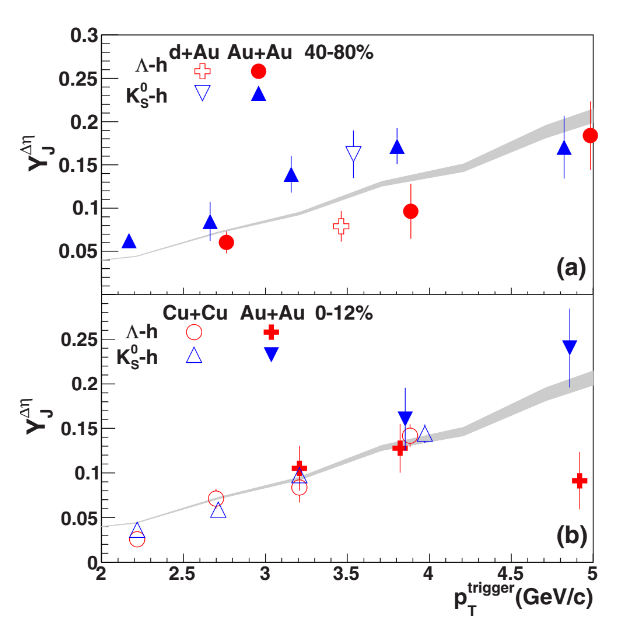
\includegraphics[scale=0.5]{./Obrazky_praca/clanokstar.png}
	\caption{Závislosť výťažkov od priečnej hybnosti identifikovanej trigrovacej častice pre 1.5 GeV/$c <p_T^{asoc}<p_T^{trig}$ v intervale $|\Delta\eta|<0,78$ ~\cite{clanokstar}}
	\label{clanokstar}
\end{figure}

\subsection{Korelácie v Pb-Pb zrážkach na experimente  ALICE na LHC}
QGP, ktorá vzniká v zrážkach relativistických ťažkých iónov, je študovaná pomocou signatúr spojených s produkciou a vlastnosťami rôznych častíc. Jednou z týchto signatúr je modifikácia jetov vplyvom QGP. Jety s istými energiami dokonca nie sú v dátovej vzorke prítomné, pretože boli absorbované plazmou. Tento jav sa nazýva "jet quenching" (z angl. - zhášanie jetov) a bol prvýkrát pozorovaný pri štúdiu dvoj\-čas\-ti\-co\-vých korelácii pri zrážkach zlato-zlato pri energii $\sqrt{s_{NN}}=$130 GeV na urýchľovači RHIC~\cite{rhic}.

V kolaborácii ALICE bolo analyzovaných 14 miliónov olovených zrážok z roku 2010 pri energii $\sqrt{s_{NN}}=$ 2.76 TeV a 37 miliónov protónových zrážok z marca 2011 pri rovnakej energii metódou dvojčasticových korelácií. Dáta boli analyzované pre intervaly $8<p^{trig}_{T}<15$ GeV/$c$ a 3 GeV/$c<p^{assoc}_{T}<p_T^{trig}$ a merali sa pomery výťažkov v centrálnych zrážkach ku výťažkom v periférnych zrážkach ($I_{CP}$) a pomery výťažkov v olovených ku protónovým zrážkam ($I_{AA}$) pre rôzne centrality \cite{clanok}. Pomer $I_{AA}$ ukazuje vplyv plazmy na konečné stavy hadrónov. 

Na obrázku~\ref{clanok2} sú zobrazené pomery $I_{AA}$ pre centrálne a periférne zrážky, pričom boli použité tri spôsoby odčítania pozadia. Potlačenie výťažku $I_{AA}\approx0.6$ pre protiľahlý pík centrálnych zrážok je považované za dôkaz straty energie v QGP. Viditeľné je aj zvýšenie pre priľahlý pík, $20-30\%$, ktoré nebolo pozorované pri nižších energiách zrážok na RHICu. Pre periférne zrážky nie sú zreteľné žiadne vplyvy plazmy, ako bolo očákavané. Podľa výsledkov tejto analýzy je pomer $I_{CP}$ v súlade s $I_{AA}$ pre centrálne zrážky (Obr.~\ref{clanok2}).



Počas tejto analýzy bolo prvý krát pozorované už skôr spomenuté navýšenie pomeru $I_{AA}$ pre centrálne zrážky, čo napovedá, že aj priľahlý partón bol ovplyvnený QGP. V publikácii~\cite{clanok} sú uvedené 3 faktory ovplyvňujúce toto navýšenie:
\begin{itemize}
	\item \textbf{zmena fragmentačnej funkcie}: vplyvom plazmy nesú hadróny v olovených zrážkach menšiu časť hybnosti pôvodného partónu ako v protónových zrážkach, čo vedie k zvýšenému počtu asociovaných častíc a $I_{AA}>1$
	\item \textbf{rôzna distribúcia počiatočných partónov}: zvýšený počet gluónov má rovnaký vplyv a vedie k potlačeniu počtu trigrovacích častíc v danom $p_T$ intervale, z čoho plynie $I_{AA}>1$
	\item \textbf{posun $p_T$ spektra partónu}: pre danú $p_T$ trigrovacej častice, mal pôvodný partón vyššiu $p_T$ v olovených zrážkach ako v protónových, čo vedie k zvýšeniu $I_{AA}$
\end{itemize}

Predpokladá sa, že všetky tri efekty hrajú úlohu a prispievajú k nameranému výsledku.

\begin{figure}[hbtp!]
	\centering
	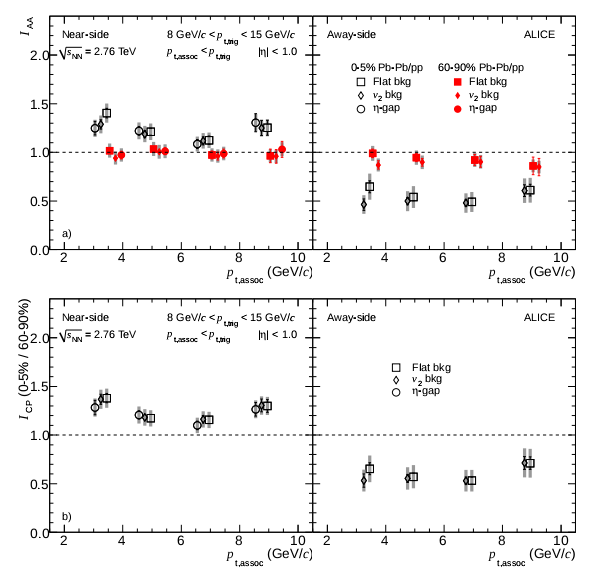
\includegraphics[scale=0.9]{./Obrazky_praca/clanok2.png}
	\caption{ Hore: $I_{AA}$ pre centrálne a periférne zrážky; dole: $I_{CP}$: Výsledky získané pomocou rôznych metód odčítania pozadia~\cite{clanok}}
	\label{clanok2}
\end{figure}

\subsection{pp a p-Pb zrážky na experimentoch CMS a ALICE}
\label{textAliceCms}
Na experimente CMS boli merané dvojčasticové korelácie v protónovo-protónových zrážkach nameraných pri energii $\sqrt{s}=$7 TeV. Celkovo bolo zanalyzovaných 150 000 zrážok, kde boli porovnávané dvojhadrónové korelácie pre "minimum bias"\footnote{Všetky detegovateľné nepružné zrážky.} zrážky a pre zrážky s vysokou multiplicitou (min. 110 zrekonštruovaných častíc). Toto porovnanie je ukázané na obr. \ref{CMSpp} pre častice so strednou priečnou hybnosťou. Pri vysokomultiplicitnej vzorke je zreteľne viditeľná štruktúra "horského hrebeňa" (ridge) v oblasti $|\Delta \phi|\approx0$ a $4>|\Delta \eta|>2$. Tento jav charakteristický pre oloveno-olovené zrážky indikujúci prítomnosť QGP bol prvýkrát pozorovaný aj v zrážkach protón-protón a žiadny z použitých MC generátorov nebol schopný tento výsledok popísať \cite{CMSpp}. 

\begin{figure}[hbtp!]
	\centering
	\begin{subfigure}{0.5\textwidth}
		\centering
		\includegraphics[width=1.\linewidth]{./Obrazky_praca/CMSppMinBias.png}
		\caption{}
	\end{subfigure}%
	\begin{subfigure}{0.5\textwidth}
		\centering
		\includegraphics[width=1.\linewidth]{./Obrazky_praca/CMSppHigh.png}
		\caption{}
	\end{subfigure}
	\caption{2D dvojčasticové korelácie pre strednú $p_{T}$ pre (a) minimum bias (b) vysoko-multiplicité prípady\cite{CMSpp}}
	\label{CMSpp}
\end{figure}

Podobná analýza bola na experimente CMS urobená aj pre zrážky protón-olovo pri energii $\sqrt{s}=5.02$ TeV, kde boli zanalyzované približne 2 milióny zrážok. Porovnávali sa tu 2D dvojhadrónové korelácie pre nízko- a vysoko-multiplicitné zrážky pre strednú $p_{T}$ (obr. \ref{CMSpPb}). Na pravom histograme pre vysoko-multiplicitné zrážky je viditeľná rovnaká "chrbtová$\mathrm{"}$ štruktúra ako pre protónovo-protónové zrážky  pre $|\Delta \phi|\approx0$  a $4>|\Delta \eta|>2$.

\begin{figure}[hbtp!]
		\centering
		\includegraphics[width=1.\linewidth]{./Obrazky_praca/CMSpPb.png}
	\caption{2D dvojčasticové korelácie pre strednú $p_{T}$ pre (a) nízko-multiplicitné a (b) vysoko-multiplicité prípady\cite{CMSpPb}}
	\label{CMSpPb}
\end{figure}

Analýza zrážok protón-olovo pri energii $\sqrt{s}=5.02$ TeV metódou dvojčasticových korelácii sa robila aj na experimente ALICE \cite{AlicepPb}. Selekciou prešlo $1,7\times10^6$ zrážok, z ktorých boli vyberané častice s priečnou hybnosťou v intervale $0.4<p_T<4$ GeV/$c$ a s pseudorapiditou $|\eta|<1.2$. Po projekcii na os $\Delta \phi$ a porovnaním výťažkov z rôznych multiplicitných binov a výťažkov z analýzy zrážok protón-protón pri $\sqrt{s}=$7 TeV sa ukázalo, že výťažky pre zrážky s vysokou multiplicitou sú výrazne väčšie ako pre tie s nízkou multiplicitou, ktoré zodpovedali výťažkom zo zrážok protón-protón (obr. \ref{ALICEpPBPhiPred}). Preto sa od dvojrozmernej korelačnej funkcie pre vysoko-multiplicitné prípady odčítala 2D korelačná funkcia pre nízko-multiplicitné prípady. Tento rozdiel je na obr. \ref{ALICErozdiel} a sú na ňom vidideľné dve kopcovité štruktúry, ktoré po projekcii na $\Delta \phi$ veľmi dobre popisuje kosínusová závislosť, ktorou boli dáta fitované. Po odčítaní tohto fitu pre jednotlivé multiplicité biny zodpovedali výťažky všetkých multiplicitných tried výťažkom zo zrážok protón-protón (obr. \ref{ALICEpPBPhiPo}).

\begin{figure}[hbtp!]
	\centering
	\begin{subfigure}{0.5\textwidth}
		\centering
		\includegraphics[width=1\linewidth]{./Obrazky_praca/ALICEpPbPred.png}
		\caption{}
		\label{ALICEpPBPhiPred}
	\end{subfigure}%
	\begin{subfigure}{0.5\textwidth}
		\centering
		\includegraphics[width=1\linewidth]{./Obrazky_praca/ALICEpPbPo.png}
		\caption{}
		\label{ALICEpPBPhiPo}
	\end{subfigure}
	\caption{Projekcia na os $\Delta \phi$ pred (a) a po (b) odčítaní pozadia s kosínusovou závislosťou získanou z fitu \cite{AlicepPb}.}
\end{figure}

\begin{figure}[hbtp!]
	\centering
	\includegraphics[width=0.7\linewidth]{./Obrazky_praca/ALICErozdiel.png}
	
	\caption{2D korelačná funkcia pre zrážky s vysokou multiplicitou po odčítaní korelačnej funkcie pre nízko-multiplicitné prípady \cite{AlicepPb}}
	\label{ALICErozdiel}
\end{figure}
Pôvod týchto štruktúr je stále otvorená otázka. Existujú viaceré modely, ktoré sa tento jav snažnia vysvetliť, zatiaľ však žiaden z nich nie je potvrdený. Jeden z modelov hovorí o miniatúrnej kvapke QGP v protónovo-protónových zrážkach a teda tieto štruktúry majú rovnaký pôvod ako v jadrovo-jadrových zrážkach. Iný model to vysvetľuje pomocou "\-opätovného spájania farieb" (colour reconnection) a  následného tvorenia toku, ktorý sa podarilo nasimulovať pomocou generátora PYTHIA8 \cite{flowPP}.

\chapter{Ciele práce} 
\begin{itemize}
	\item Vypracovanie všeobecného programu použiteľného na analýzu identifikovaných a neidentifikovaných dvojhadrónových korelácií na všetky typy zrážok pri rôznych energiách
	\item Aplikovanie kódu na dáta z protónovo-protónových zrážok pri 13 TeV (vysoká štatistika, nízke pozadie)
	\begin{itemize}
		\item Testovanie metódy na h-h koreláciach
		\item Analýza korelácií s identikovanými trigrovacími časticami (podivné častice)
		\item MC closure test
		\item Výpočet výťažkov v závislosti od priečnej hybnosti trigrovacích častíc a multiplicity zrážok
		\item Porovnanie výsledkov s MC vygenerovanými dátami 
	\end{itemize}
\end{itemize}


\chapter{Metóda merania}

\section{Experiment ALICE}

ALICE (z anglického A Large Ion Collider Experiment – experiment na Veľkom iónovom zrážači) je jedným zo štyroch veľkých experimentov na LHC v CERNe. Zameriava sa najmä na výskum partónovej hmoty vznikajúcej v zrážkach ultrarelativistických ťažkých iónov. Táto hmota sa svojimi vlastnosťami podobá na teoreticky predpovedanú QGP, ktorou bol tvorený Vesmír tesne po Veľkom Tresku. V podmienkach LHC to zodpovedá približne 1 miliardtine sekundy veku Vesmíru.

Detektor  ALICE umožňuje detekciu rôznych druhov častíc pri zrážkach protón - protón, ale predovšetkým umožňuje štúdium zrážok olovo - olovo pri extrémnych podmienkach (vysoká teplota, tlak a energia). Jeho rozmery dosahujú $16\times 16\times26 \rm{m^3}$ s váhou približne 10,000 ton~\cite{alice}. Valcová časť detektora je umiestnená v solenoidálnom magnetickom poli s indukciou 0.5 T, ktoré spôsobuje zakrivenie dráh.

Experiment ALICE je tvorený viacerými detektormi, ako je zobrazené na obrázku \ref{ALICE}. Každý z jednotlivých subdetektorov využíva inú technológiu a má svoju nezastupiteľnú úlohu v celom detektorovom komplexe. Pri analýze podivných častíc hrajú nezastupiteľnú úlohu detektory ITS, V0 a TPC.

\begin{figure}[hbtp!]
	\begin{center}
		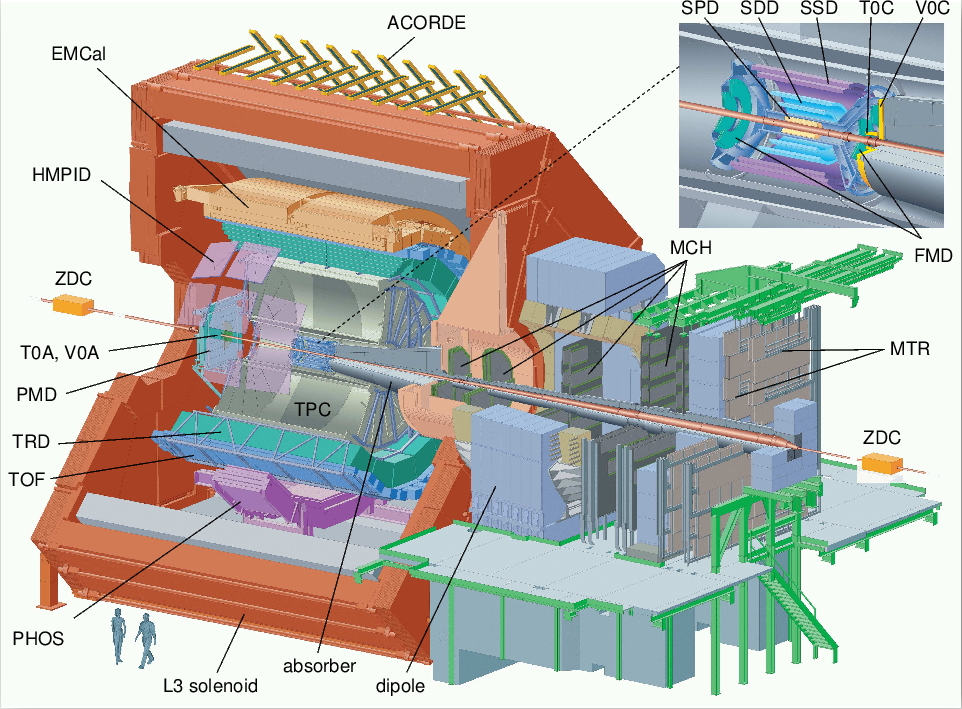
\includegraphics[width=0.9\textwidth]{./Obrazky_praca/ALICE.png}
		\caption{Experiment ALICE skladajúci sa z viacerých subdetektorov~\cite{aliceDetektor}}
		\label{ALICE}
	\end{center}
\end{figure}

\subsection{Vnútorný dráhový systém}

ITS (z anglického Inner Tracking System) je systém najvnútornejších detektorov, ktorý sa nachádza blízko miesta zrážky, a teda v oblasti s vysokou hustotou častíc (pre zrážky olovo-olovo až 50 dráh na $\mathrm{cm}^2$ ). Je tvorený šiestimi vrstvami kremíkových detektorov, ktoré slúžia najmä na detekciu primárneho vertexu, určovanie sekundárneho vertexu slabých rozpadov a určovanie a rozlišovanie dráh jednotlivých častíc. Pokrýva peudorapiditný interval $|\eta|<0,9$.

\subsection{V0 detektor}

 V0 je tvorený dvoma kruhovými časťami (V0A a V0C), pričom každá z nich sa náchadza na jednej strane ITS. Každý z kruhov je tvorený 32 scintilačnými detektormi. V0 detektory pokrývajú preudorapiditné intervaly $2,8?
 <\eta<5,1$ (V0A) a $-3,7<\eta<-1.7$ (V0C). Jeho hlavnou úlohou je "triggering"\footnote{Tigger je elektronický systém, ktorý na základe signálov z detektorov rozhoduje, či došlo k fyzikálne zaujímavej zrážke, ktorá bude uložená na grid a následne spracovávaná.} pre centrálne barelové detektory a vďaka monotónnej závislosti počtu detekovaných častíc od počtu primárne emitovaných častíc v zrážke je užitočným detektorom na určovanie centrality zrážok pomocou určovania multiplicity zrážok.  

\subsection{Časovo-projekčná komora}
\label{textTPC}
Na pozorovanie dráh nabitých častíc produkovaných v zrážkach slúžia dráhové detektory. Hlavný z nich je TPC (z anglického Time Projection Chamber - časovo projekčná komora).

TPC je valec naplnený plynovou zmesou ( $Ne/CO_2/N_2$) s objemom $88m^3$ (obr.~\ref{tpc}) rozdelený centrálnou elektródou na dve driftovacie časti. Pozdĺž z-ovej osi je udržiavané rovnomerné elektrické pole o veľkosti 100kV. Nabité častice pri svojej ceste ionizujú plyn v TPC. Tým sú uvoľňované elektróny z molekúl plynu, ktoré po krátkom vychýlení následne driftujú k anódam na okraji valca. Na základe informácie o čase driftu elektrónov a o mieste ich dopadu sa rekonštruujú body v priestore, cez ktoré častica preletela. Signál je zosilnený lavínovým efektom v blízkosti anódy~\cite{TPCobr}, ktorá je tvorená mnohovláknovými proporcionálnymi komorami. Tie sú rozdelené na 18 sektorov v azimutálnom uhle a na 2 sektory v radiálnom smere. Homogénne magnetické pole v smere osi z, v ktorom je celý detektor umiestnený, umožňuje určenie hybnosti a elektrického náboja častíc. Z informácií o energetických stratách v TPC a v iných detektoroch je možné určiť aj druh častice. 

\begin{figure}[hbtp!]
	\begin{center}
	 	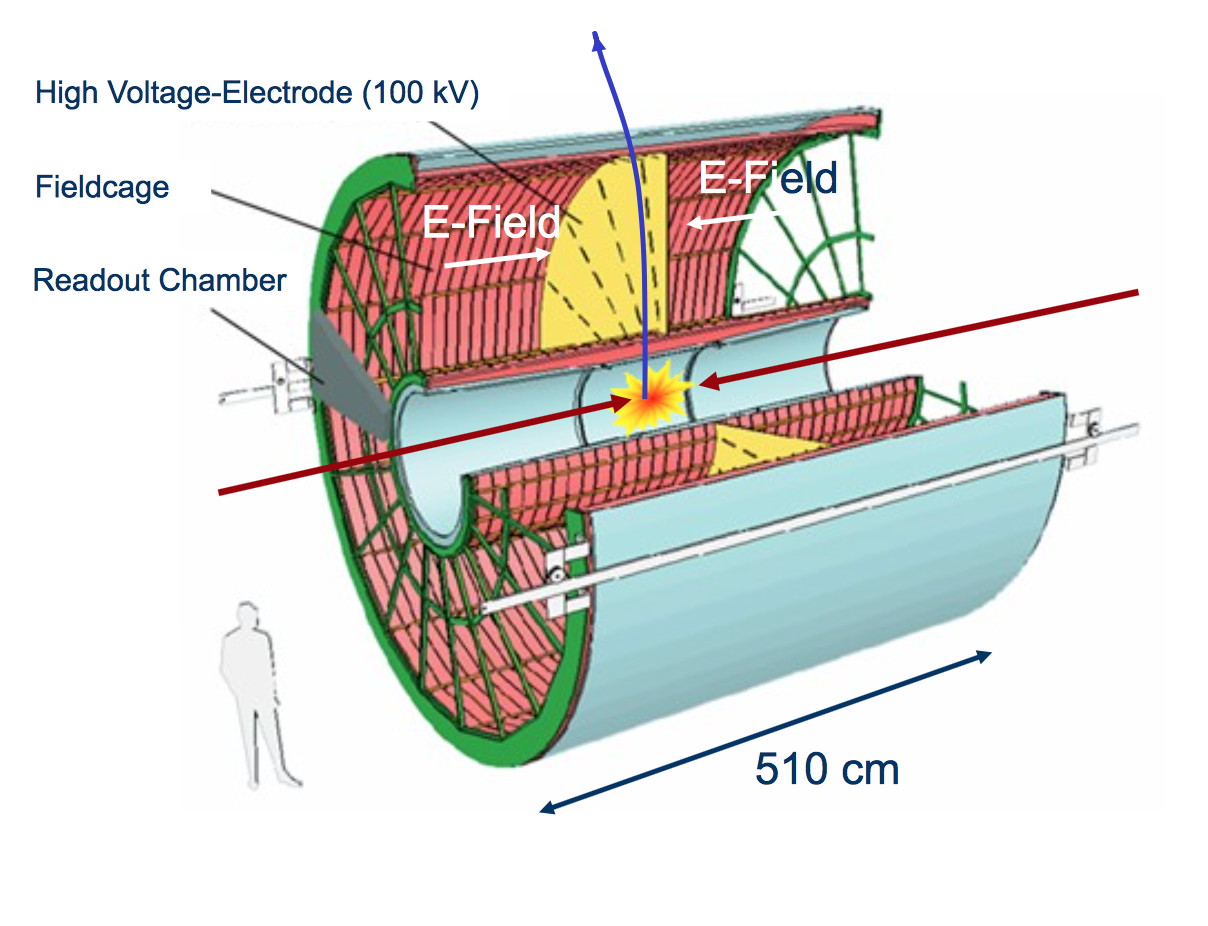
\includegraphics[width=0.7\textwidth]{./Obrazky_praca/tpc.png}
		\caption{Porovnanie veľkosti TPC s veľkosťou človeka~\cite{TPCobr}.}
		\label{tpc}
	\end{center}
\end{figure}

\section{ROOT}
ROOT je vývojové prostredie napísané v objektovo orientovanom programovacom jazyku C++ určené na analýzu dát. Užívateľovi poskytuje veľký počet funkcionalít spojených so spracovávaním veľkého množstva dát, napr. histogramy, funkcie pre štatistickú analýzu, vizualizáciu zrážok a bohatý matematický aparát. Užívateľ má taktiež možnosť vytvorenia vlastných tried a knižníc vhodných pre svoju analýzu. ROOT je možné prepojiť s už existujúcimi programovacími jazykmi a štatistickými programami, ako sú Python, Ruby, R a Mathematica~\cite{root}.

\section{AliRoot}
AliRoot \cite{aliroot} je oficiálnym analyzačným softvérom kolaborácie ALICE, základom kto\-ré\-ho je ROOT rozšírený o špeciálne triedy, ktoré sa používajú na rekonštrukciu, simuláciu a analýzu dát v experimente ALICE. Jeho štruktúra, triedy a funkcie sú vytvárané v súlade s~potrebami analýzy dát nameraných na experimente ALICE. Z toho vyplýva aj delenie jeho tried na všeobecné a triedy využívané pre rekonštrukcii, simulácii a analýze. 

Pomocou AliRootu je možné spracovávať dáta v rôznych formátoch:
\begin{itemize}
	\item \textbf {raw dáta} - signály z jednotlivých detektorov priradené k jednotlivým zrážkam, ktoré sa ďalej spracovávajú na gride\footnote{Grid je celosvetová počítačová sieť, na ktorej sa rekonštruujú a analyzujú dáta. Grid experimentu ALICE sa nazýva AliEn a obsahuje okolo 100000 CPU jadier.} 
	\item \textbf {ESD (Event Summary Data) dáta} - spracované ale nefiltrované raw dáta, obsahujú objekty, ktoré sa vypočítali pomocou raw dát, ako napríklad druhy nabitých častíc alebo slabé neutrálne rozpady. K jednotlivým objektom sú priradené ich vlastnosti ako hmotnosť, hybnosť, energia, elektrický náboj a pod..
	\item \textbf {AOD (Analysis Object Data) dáta} - filtrované ESD dáta vhodné skoro pre všetky druhy analýz, tvoria približne 10\% pôvodnej veľkosti ESD dát, použité aj v tejto analýze
\end{itemize}

Pre všetky tieto druhy dát sú v AliRoote vytvorené špeciálne triedy s podobnými funkciami. Okrem dát zozbieraných z detektorov, AliRoot umožňuje spracovanie aj simulovaných dát, pre ktoré tiež existujú samostatné triedy. Na simulácie sa využívajú rôzne Monte Carlo (MC) generátory zrážok:
\begin{itemize}
	\item HIJING \cite{hijing} - generovanie jadrovo-jadrových zrážok, založený na QCD a Lundskom modeli fragmentácie jetov
	\item PYTHIA \cite{pythia}, PHOJET \cite{phojet}, Herwig \cite{herwig} - generovanie protónovo-protónových zrážok
\end{itemize}

Rekonštrukcia simulovaných dát (raw, ESD, AOD) sa uskutočňuje pomocou rovnakého kódu ako rekonštrukcia reálnych dát.

\chapter{Výsledky}

\section{Spracované dáta a selekčné kritéria}
V analýze boli spracovávané dáta z protónovo-protónových zrážok pri energii $\sqrt{s_{NN}}=13$~TeV z roku 2015. Analyzované dáta boli vo formáte AOD. Dokopy bolo analyzovaných $1.17\times10^7$ zrážok, ktoré boli vyselektované na základe tzv. minimum bias trigra, ktorý znamená lkoincidenciu medzi signálmi z detektorov V0A a V0C.
MC produkcia bola zviazaná s týmito dátami\footnote{Podmienky, pri ktorých boli zbierané dáta, boli implementované aj do nastavení simulácie. } a boli použité MC produkcie z 3 rôznych generátorov: PYTHIA6 - Perugia \cite{perugia} , PYTHIA8 - Monash \cite{monash}, EPOS - LHC \cite{epos}. 

Analyzované boli iba tie zrážky, ktorých PV bol vzdialený maximálne 10 cm od geometrického stredu detektora. Nabité primárne hadróny museli spĺňať základné detektorové selekčné kritériá pre TPC a ITS. Navyše ich najkratšia vzdialenosť od PV v rovine xy mohla byť najviac 2,4 cm a smere rovnobežnom so zväxkom maximálne 3,2 cm a zároveň tieto dve vzdialenosti museli spadať do vnútra elipsy definovanej maximálnymi vzdialenosťami. Dráha rekonštruovaná v TPC a spojená a PV mohla mať $\chi ^2$ maximálne 36 a podiel zdieľaných klastrov ku celkovému počtu klastrov v TPC musel byť meší ako 0,4. Pre danú dráhu bol navyše vyžadovaný záznam z SPD\footnote{Silicon Pixel Detector - najvnútornejšia časť ITS. } a musela byť vypočítana celá dráha v ITS smerujúca z PV.

Na obrázku~\ref{schema} je zobrazená schéma rozpadu $V^0$ častice, konkrétne $\Lambda$ na dve dcérske častice $p+\pi^{-}$. Pri selekcii jednotlivých $V^0$ častíc sme sa zamerali na parametre:
\begin{itemize}
	\item DCA (Distance of Closest Approach) $V^0$ Neg. daughter - najkratšia vzdialenosť v priestore negatívne nabitej dcéry k primárnemu vertexu
	\item DCA $V^0$ pos. - najkratšia vzdialenosť pozitívne nabitej dcéry
	\item DCA between daughters - najkratšia vzdialenosť v priestore medzi dcérami $V^0$ častice
	\item V0 2D Decay Radius  - vzdialenosť bodu rozpadu $V^0$ (sekundárny vertex) a primárneho vertexu zrážky v $xy$ rovine
	\item Pointing angle $\theta_{PA}$ - uhol medzi vektorom celkovej hybnosti $V^0$ častice a úsečkou spájajúcou primárny vertex zrážky s bodom rozpadu $V^0$ 
	\item lifetime - vzdialenosť, ktorú prejde daná častica počas svojej doby života
	\item pseudorapidita $\eta$
\end{itemize} 
Všetky hodnoty selekčných kritérii sú zosumarizované v tabuľke~\ref{tabulka}.

\begin{figure}[hbtp!]
	\centering
	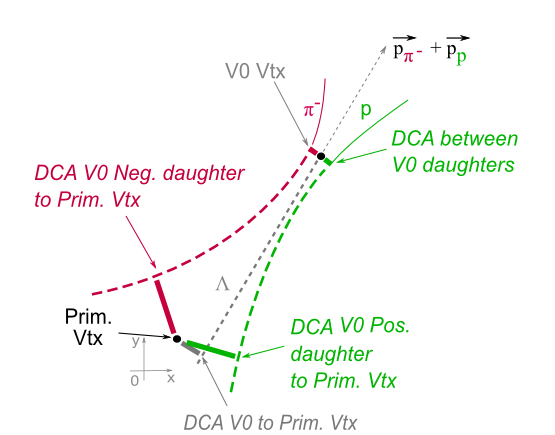
\includegraphics[scale=0.8]{./Obrazky_praca/SchemaV0.png}
	\caption{Schéma topologickej selekcie pre $V^0$ častice~\cite{schema}}
	\label{schema} 
\end{figure}

\begin{table}[hbtp!]
	\begin{center}
		\begin{tabular}{|c|c|}
			\hline
			 \multicolumn{2}{|c|}{Selekčné kritéria pre $V^{0}$}  \\ \hline
			$K^0_S$ & $\Lambda$ + $\bar{\Lambda}$ \\ \hline
			$cos\theta_{PA} >0.97$ & $cos\theta_{PA} >0.995$  \\ \hline
			$|\eta|<0.8$ & $|\eta|<0.8$   \\ \hline
			DCA Neg$>$0.06 cm & DCA Neg$>$0.06 cm \\ \hline
			DCA Pos$>$0.06 cm & DCA Pos$>$0.06 cm \\ \hline
			DCA V0 daughters$<$ 1 cm & DCA V0 daughters $<$1 cm \\ \hline
			lifetime$<$20 cm & lifetime$<$30 cm \\ \hline
			V0 2D Decay Radius $>$ 0.5 & V0 2D Decay Radius $>$ 0.5\\ 
			\hline
		\end{tabular}
		\caption{Tabuľka selekčných kritérii pre $V^{0}$ častice}
		\label{tabulka}
	\end{center}
\end{table}
\newpage
Selekčné kritéria boli aplikované aj na dcérske častice pochádzajúce z $V^0$. Rekonštruované dráhy nabitých dcérskych častíc $V^0$ prešli najmenej cez 70 čítacích rovín ("padrows") v TPC. Pomer počtu reálne prejdených a teoreticky možných rovín v TPC musel byť väčší ako 0.8. Posledným kritériom výberu dcérskych častíc bola ich identifikácia pomocou straty energie v TPC pre $V^0$ častice s priečnou hybnosťou menšou ako 1 GeV, kde strata energie kandidáta na dcérsku časticu $V^0$ musela byť v intervale do $3\sigma$ od teoreticky vypočítanej straty energie pre danú časticu.

Na základe týchto selekčných kritérii sme z rozdelenia invariatnej hmotnosti dcérskych častíc $V^0$ vybrali kandidátov $V^{0}$ do korelačnej analýzy v intervaloch (0,48-0.,2) Gev/$c^{2}$ pre $K^{0}_{S}$ (obr. \ref{k0}) a (1,1-1,3) GeV/$c^{2}$ pre $\Lambda$ a $\bar{\Lambda}$ (obr.\ref{Lambdy} ). 

\begin{figure}[hbtp!]
	\centering
	\includegraphics[scale=0.4]{../histogramy/massK0.png}
	\caption{Vybratý kandidáti na mezón $K^0_S$ z invariantného rozdelenia párov $\pi^+\pi^-$}
	\label{k0}
\end{figure}
\begin{figure}
	\centering
	\begin{subfigure}{0.5\textwidth}
		\centering
		\includegraphics[width=1\linewidth]{../histogramy/massLam.png}
		\caption{}
		\label{Lam}
	\end{subfigure}%
	\begin{subfigure}{0.5\textwidth}
		\centering
		\includegraphics[width=1\linewidth]{../histogramy/massALam.png}
		\caption{}
		\label{ALam}
	\end{subfigure}
	\caption{Vybrantý kandidáti na baryón (a) $\Lambda$ z invariantného rozdelenia párov $p\pi^-$, (b) $\bar{\Lambda}$ z invariantného rozdelenia párov $\bar{p}\pi^+$}
	\label{Lambdy}
\end{figure}

Posledným kritériom potrebným na štúdium dvojčasticových korelácií je priečna hybnosť. Trigrovacia častica musela mať priečnu hybnosť väčšiu ako 4 GeV/$c$ a asociovaná sa musela nachádzať v intervale 2 GeV/$c<p_T^{asoc}<p_T^{trig}$.

\section{Korekcie}
Okrem jednotlivých selekčných kritérii bolo potrebné pri analýze použiť aj tri typy korekcií. 

Prvou je korekcia na konečnú akceptanciu detektora. Túto korekciu sme urobili pomocou metódy mixing. Trigrovacia častica bola z jedného prípadu a asociovaná častica z iného nezávislého prípadu. Kvôli väčšej štatistike sme jednu trigrovaciu časticu mixovali s minimálne piatimi prípadmi, pričom oba prípady museli mať z-ovú zložku primárneho vertexu rovnakú v rámci 1 cm a mať približne rovnakú multiplicitu. Mixovaním získané rozdelenie tvaru kombinatorického pozadia v rovine ($\Delta \phi \Delta \eta$) je na obrázku~\ref{pozadie}. Toto rozdelenie bolo následne normované na hodnotu najvyššieho binu rozdalenia. Za predpokladu, že účinnosť rekonštrukcie páru v najvyššom bine je 100\%, získame tak rozdelenie účinnosti rekonštrukcie párov v priestore $(\Delta \phi,\Delta\eta)$.

\begin{figure}[hbtp!]
	\centering
	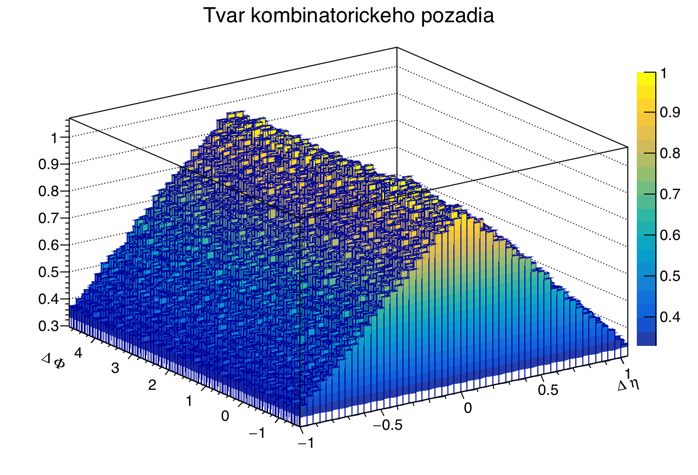
\includegraphics[scale=0.5]{./Obrazky_praca/pozadie.png}
	\caption{Príklad tvaru kombinatorického pozadia, t.j. častice v páre spolu fyzikálne nesúvisia, pri dvojčasticových koreláciách namodelovaného metódou mixing}
	\label{pozadie}
\end{figure}

Druhou je korekcia na účinnosť rekonštrukcie asociovaných častíc v detektore. Pri tejto korekcii boli použité dáta nasimulované metódou Monte Carlo, ktoré zodpovedajú energii aj druhu zrážok spracovávaných dát. Generované dáta prešli re\-kon\-štruk\-ciou, pri ktorej boli použité rovnaké selekčné kritéria ako pre reálne dáta. Účinnosť re\-kon\-štruk\-cie sa definuje ako podiel počtu zrekonštruovaných častíc ku počtu generovaných v závislosti od priečnej hybnosti, pseudorapidity asociovanej častice a z-ovej súradnice primárneho vertexu, pričom každá rekonštruovaná častica musí byť prepojená s generovanou časticou, t.j. nebolo možné zrekonštruvať časticu, ktorá nebola pre danú zrážku vygenerovaná.  
\begin{equation}
\footnotesize
\epsilon_{asoc}(p_{T}^{asoc},\eta^{asoc},Pz) = \frac{N_{asoc}^{rek}}{N_{asoc}^{gen}}(p_{T}^{asoc},\eta^{asoc},Pz)
\end{equation}
Poslednou je korekcia na účinnosť rekonštrukcie trigrovacích častíc\footnote{Takáto korekcia na účinnosť rekonštrukce trigrovacích častíc bola robená aj v predchádzajúcich korelačných analýzach \cite{Jan-Fiete}}. Bola robená podobne ako pre asociované častice v závislosti od priečnej hybnosti, pseudorapidity trigrovacej častice a z-ovej súradnice primárneho vertexu. 
\begin{equation}
\footnotesize
\epsilon_{trig}(p_{T}^{trig},\eta^{trig},Pz) = \frac{N_{trig}^{rek}}{N_{trig}^{gen}}(p_{T}^{trig},\eta^{trig},Pz)
\end{equation}
\begin{equation}\end{equation}
Na obrázku \ref{uc} je zobrazená účinnosť rekonštrukcie pre jednotlivé typy častíc v závislosti od ich priečnej hybnosti. Po aplikovaní všetkých korekcií dostávame výsledné dvojrozmerné rozdelenie, ktoré ešte normujeme na počet trigrovacích častíc:
\begin{equation}
\footnotesize
\frac{d^2N^{corrected}_{pair}}{d\Delta\phi d\Delta\eta}(\Delta\phi,\Delta \eta)=
\frac{1}{N^{corr}_{trig}} \frac{d^2N^{raw}_{pair}}{d\Delta\phi d\Delta\eta} \frac{1}{\epsilon_{asoc}(p_{T}^{asoc},\eta^{asoc},Pz)}\frac{1}{\epsilon_{pair}(\Delta\phi,\Delta\eta)}
\frac{1}{\epsilon_{trig}(p_{T}^{trig},\eta^{trig},Pz)}
\end{equation}
\begin{equation}
\footnotesize
N^{corr}_{trig}=N^{raw}_{trig}\frac{1}{\epsilon_{trig}(p_{T}^{trig},\eta^{trig},Pz)}
\end{equation}

\begin{figure}[hbtp!]
	\centering
	\includegraphics[scale=0.4]{../histogramy/vytazky/ucinnost.png}
	\caption{Účinnosť rekonštrukcie jednotlivých častíc v závislosti od ich priečnej hybnosti}
	\label{uc}
\end{figure}

\section{MC closure test}

Monte Carlo closure test je v princípe skúška správnosti kódu použitého na štúdium dvojčasticových korelácií. Použitá tu bola kombinácia dvoch produkcií MC (Perugia a Monash) kvôli zvýšeniu štastistiky. V rámci tohto testu sa pozeráme na korelačné \-funk\-cie hadrónov, ktoré boli vygenerované a na korelačné funkcie MC zrekonštruovaných hadrónov, na ktoré boli aplikované už skôr spomínané korekcie. Pre generované ako aj rekonštruované dáta sme urobili korelačné funkcie v závislosti od priečnej hybnosti  a od druhu trigrovacej častice. Následne sme tieto dvojrozmerné rozdelenia generovaných častíc predelili rozdeleniami rekonštruovaných častíc. Z týchto dvojrozmerných pomerov sme potom robili projekcie na jednotlivé osi, pričom prázdne biny boli ignorované, a tie sme fitovali konštantnou funkciou. Hodnoty jednotlivých fitov sme zobrazili v závislosti od priečnej hybnosti a druhu trigrovacej častice na obr. \ref{fitMC} . 

Ak boli všetky použité korekcie správne a dostatočne presné, výsledok by sa mal nachádzať v blízkom okolí 1, ktorý sme dosiahli pre korelácie, kde trigrovacími časticami boli nabité hadróny. Tento výsledok znamená, že s aplikovanými korekciami sme dokázali zrekonštruovať reálnu zrážku, len minimálne ovplyvnenú detektorom.
V prípade $V^0$ ako trigrovacích častíc je fit viac posunutý od 1. Ako je vidieť na jednotlivých projekciách (Obr. \ref{K0phi}  až Obr.\ref{heta}  ), projekcia na $\Delta \phi$ je približne konštantná a rovnako posunutá od hodnoty 1 pre $K^0_S$ ako aj pre $\Lambda$. Pri projekcii na $\Delta \eta$ vidíme rovnaké správanie v okolí 0, teda v okolí korelačného píku, ale na okrajoch hodota pomeru klesá. Tento efekt by mohol byť spôsobený detektorom a mal by sa zohľadniť pri výpočte systematickej chyby. 

\begin{figure}
	\centering
	\begin{subfigure}{0.5\textwidth}
		\centering
		\includegraphics[width=1.1\linewidth]{../histogramy/PorovnanieMC/Projekcie/fitPhi.png}
		\caption{}
		\label{fitPhi}
	\end{subfigure}%
	\begin{subfigure}{0.5\textwidth}
		\centering
		\includegraphics[width=1.1\linewidth]{../histogramy/PorovnanieMC/Projekcie/fitEta.png}
		\caption{}
		\label{fitEta}
	\end{subfigure}
	\caption{Hodnota fitu pre jednotlivé $p_{T}^{trig}$ biny.}
	\label{fitMC}
\end{figure}

\begin{figure}
	\centering
	\includegraphics[width=1\linewidth]{../histogramy/PorovnanieMC/Projekcie/15a+c_K0_phi.png}
	\caption{Projekcia na os $\Delta \phi$ pre korelácie $K^0_S - h$}
	\label{K0phi}
\end{figure}

\begin{figure}
	\centering
	\includegraphics[width=1\linewidth]{../histogramy/PorovnanieMC/Projekcie/15a+c_K0_eta.png}
	\caption{Projekcia na os $\Delta \eta$ pre korelácie $K^0_S - h$}
	\label{K0eta}
\end{figure}
\begin{figure}
\centering
\includegraphics[width=1\linewidth]{../histogramy/PorovnanieMC/Projekcie/15a+c_Lam_phi.png}
\caption{Projekcia na os $\Delta \phi$ pre korelácie $(\Lambda + \bar{\Lambda})- h$}
\label{Lamphi}
\end{figure}
\begin{figure}
	\centering
	\includegraphics[width=1\linewidth]{../histogramy/PorovnanieMC/Projekcie/15a+c_Lam_eta.png}
	\caption{Projekcia na os $\Delta \eta$ pre korelácie $(\Lambda + \bar{\Lambda})- h$}
	\label{Lameta}
\end{figure}

\begin{figure}
	\centering
	\includegraphics[width=1\linewidth]{../histogramy/PorovnanieMC/Projekcie/15a+c_hh_phi.png}
	\caption{Projekcia na os $\Delta \phi$ pre korelácie $h - h$}
	\label{hphi}
\end{figure}

\begin{figure}
	\centering
	\includegraphics[width=1\linewidth]{../histogramy/PorovnanieMC/Projekcie/15a+c_hh_eta.png}
	\caption{Projekcia na os $\Delta \eta$ pre korelácie $h - h$}
	\label{heta}
\end{figure}



\section{Výťažky}

Na získanie výťažkov sme najprv z dvojrozmerného rozdelenia $\frac{d^2N}{d\Delta \phi d\Delta \eta}$, ktoré bolo podelené rozdelením získaným z metódy mixing a korigované na efektivitu rekonštrukcie asociovaných aj trigrovacích častíc, projektovali jednorozmerné histogra\-my pozdĺž osi $\Delta\phi$ pre rôzne intervaly priečnej hybnosti trigrovacej častice pre jednotlivé druhy trigrovacích častíc. Keďže medzi  výsledkami pre trigrovacie častice $\Lambda$ a $\bar{\Lambda}$ neboli viditeľné žiadne signifikantné rozdiely, ich rozdelenia boli spojené kvôli zmenšeniu štatistických chýb. Jednorozmerné rozdelenia sme následne normovali na počet trigrovacích častíc, ktorý bol taktiež korigovaný na efektivitu rekonštrukcie. 

Pozadie sme určovali pomocou konštantnej funkcie. Jej hodnota bola vypočítana ako aritmetický priemer hodnoty rozdelenia v troch binoch okolo 1 a troch binoch okolo $-1$. Výsledné rozdelenia sú zobrazené na obrázkoch \ref{K0} až \ref{hh}. 

\begin{figure}[hbtp!]
	\centering
	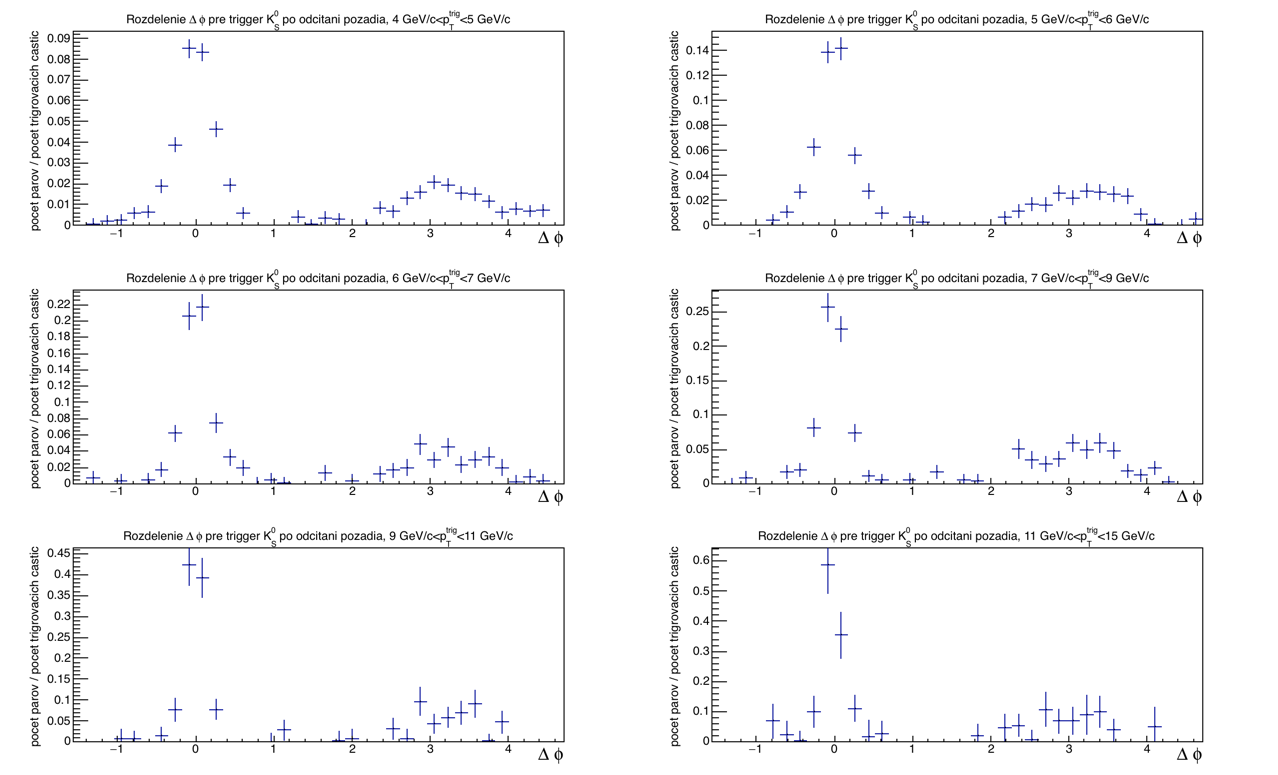
\includegraphics[width=\textwidth]{./Obrazky_praca/DeltaPhiKH.png}
	\caption{Rozdelenie $\Delta \phi$ pre trigrovaciu časticu $K^0_S$ po odčítaní pozadia pre rôzne intervaly $p_T^{trig}$}
	\label{K0}
\end{figure}

\begin{figure}[hbtp!]
	\centering
	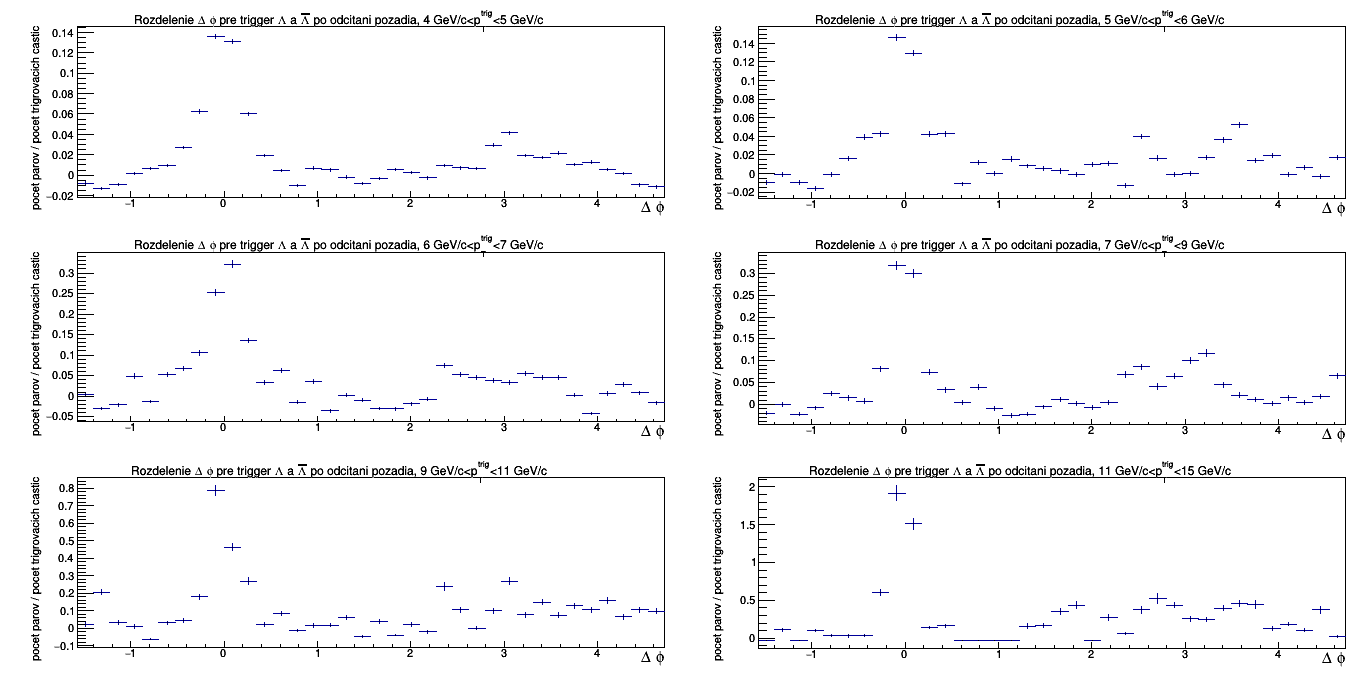
\includegraphics[width=\textwidth]{./Obrazky_praca/DeltaPhiLH.png}
	\caption{Rozdelenie $\Delta \phi$ pre pre trigrovacie častice $\Lambda$ a $\bar{\Lambda}$  po odčítaní pozadia pre rôzne intervaly $p_T^{trig}$}
	\label{lambda}
\end{figure}

\begin{figure}[hbtp!]
	\centering
	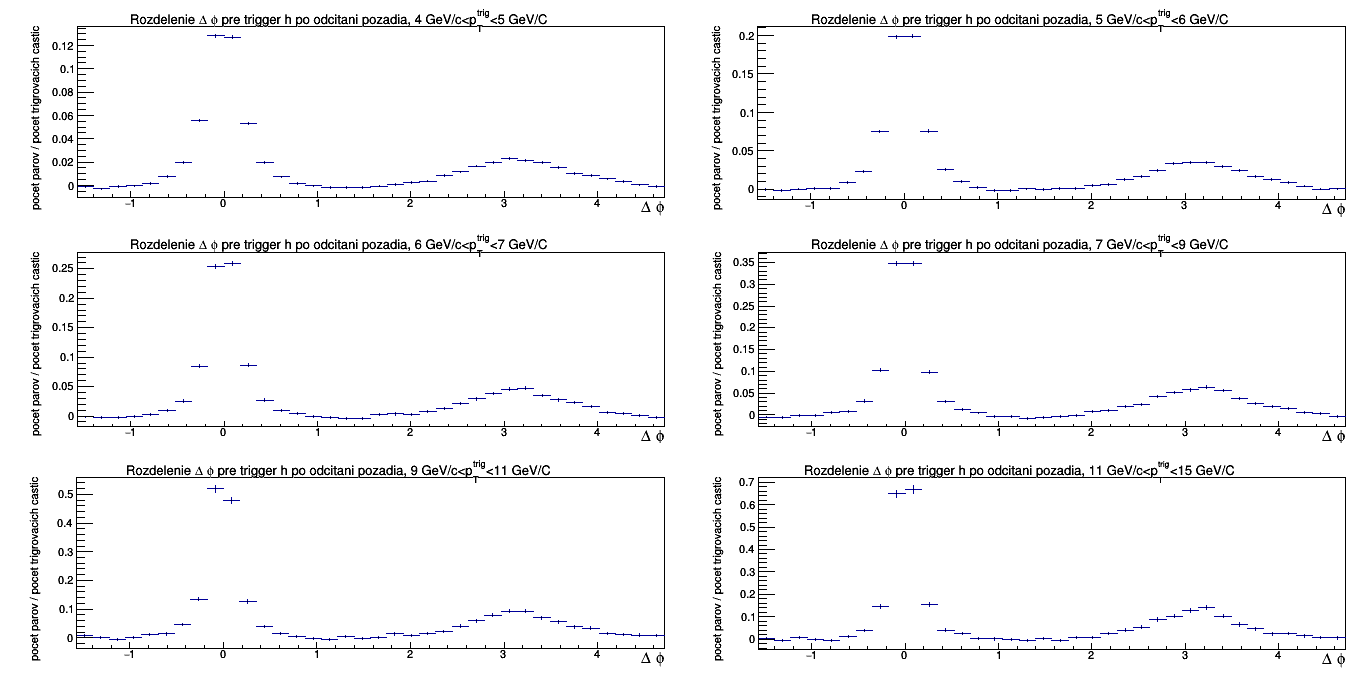
\includegraphics[width=\textwidth]{./Obrazky_praca/DeltaPhiHH.png}
	\caption{Rozdelenie $\Delta \phi$ pre nabitý hadrón ako trigrovaciu časticu po odčítaní pozadia pre rôzne intervaly $p_T^{trig}$}
	\label{hh}
\end{figure}
\newpage

Výťažky sme počítali pomocou vzťahu~\ref{yield} v intevale $-0.9$ až 0.9 pre priľahlý pík a v intervale $\pi\pm1.5$ pre protiľahlý pík. Závislosti výťažkov pre priľahlý a protľahlý pík od priečnej hybnosti trigrovacej častice sú zobrazené na obrázkoch \ref{near} a \ref{away}.

\begin{figure}[hbtp!]
	\centering
	\includegraphics[width=0.8\textwidth]{./Obrazky_praca/vytazky_minBias_prilahly_mult.png}
	\caption{Závislosť výťažkov od priečnej hybnosti trigrovacej častice pre priľahlý pík}
	\label{near}
\end{figure}

\begin{figure}[hbtp!]
	\centering
	\includegraphics[width=0.8\textwidth]{./Obrazky_praca/vytazky_minBias_protilahly_mult.png}
	\caption{Závislosť výťažkov od priečnej hybnosti trigrovacej častice pre protiľahlý pík}
	\label{away}
\end{figure}

\subsection{Výťažky a korelačné funkcie v závislosti od multiplicity zrážok}
Okrem závislosti výťažkov od priečnej hybnosti trigrovacej častice sme študovali aj závislosti výťažkov pre jednotlivé trigrovacie častice aj od multiplicity zrážok. Zrážky sme rozdelili na 3 kategórie: 0-10\% - zrážky s najvyššou multiplicitou (viac ako 11,5 $\braket{dN_{ch}/d\eta>}$\footnote{Priemerný počet nabitých častíc na jednotku pseudorapidity pre strednú pseudorapiditu.}), 10-50\% - zrážky so strednou multiplicitou (4,5 - 11,5 $\braket{dN_{ch}/d\eta}$) a 50-100\% - zrážky s nízkou multiplicitou (menej ako 4,5 $\braket{dN_{ch}/d\eta}$) a v každej sme vypočítali výťažky v závislosti priečnej hybnosti trigrovacej častice pre jednotlivé druhy korelácií (obr. \ref{K0mult} až \ref{hhmult}).
\begin{figure}
	\centering
	\begin{subfigure}{0.5\textwidth}
		\centering
		\includegraphics[width=1.\linewidth]{./Obrazky_praca/vytazky_Kh_prilahly_mult.png}
		\caption{}
		\label{K0pril}
	\end{subfigure}%
	\begin{subfigure}{0.5\textwidth}
		\centering
		\includegraphics[width=1.\linewidth]{./Obrazky_praca/vytazky_Kh_protilahly_mult.png}
		\caption{}
		\label{K0proti}
	\end{subfigure}
	\caption{Závislosť výťažkov pre korelácie $K^0_S - h$ od $p_T^{trig}$ a multiplicitnej triedy zrážky pre priľahlý pík (a) a protiľahlý pík (b).}
	\label{K0mult}
\end{figure}
\begin{figure}
	\centering
	\begin{subfigure}{0.5\textwidth}
		\centering
		\includegraphics[width=1.\linewidth]{./Obrazky_praca/vytazky_Lh_prilahly_mult.png}
		\caption{}
		\label{Lampril}
	\end{subfigure}%
	\begin{subfigure}{0.5\textwidth}
		\centering
		\includegraphics[width=1.\linewidth]{./Obrazky_praca/vytazky_Lh_protilahly_mult.png}
		\caption{}
		\label{Lamproti}
	\end{subfigure}
	\caption{Závislosť výťažkov pre korelácie $(\Lambda + \bar{\Lambda})- h$ od $p_T^{trig}$ a multiplicitnej triedy zrážky pre priľahlý pík (a) a protiľahlý pík (b).}
	\label{Lammult}
\end{figure}
\begin{figure}
	\centering
	\begin{subfigure}{0.5\textwidth}
		\centering
		\includegraphics[width=1.\linewidth]{./Obrazky_praca/vytazky_hh_prilahly_mult.png}
		\caption{}
		\label{hhpril}
	\end{subfigure}%
	\begin{subfigure}{0.5\textwidth}
		\centering
		\includegraphics[width=1.\linewidth]{./Obrazky_praca/vytazky_hh_protilahly_mult.png}
		\caption{}
		\label{hhproti}
	\end{subfigure}
	\caption{Závislosť výťažkov pre korelácie $h - h$ od $p_T^{trig}$ a multiplicitnej triedy zrážky pre priľahlý pík (a) a protiľahlý pík (b).}
	\label{hhmult}
\end{figure}

Podobne ako sa robilo \cite{AlicepPb}, skúsili sme porovnať dvojrozmerné korelačné funkcie pre jednotlivé multiplicitné triedy zrážok. Na obr. \ref{multroz} je zobrazený rozdiel korelačných funkcií pre triedu najvyšších a najnižších multiplicitných tried ((0-10\%)-(50-100\%)).

Aby sme lepšie porovnali veľkosti výťažkov pre zrážky s najvyššou a najnižšou multiplicitou urobili sme pomer $I_{CP}$, kde sme delili výťažky vysokomultiplicitých zrážok výťažkami  z nízkomultiplicitných zrážok. Tento pomer v závislosti od priečnej hybnosti trigrovacej častice pre priľahlý aj protiľahlý pík je zobrazený na obr. \ref{Icpnase}. 

\begin{figure}[hbtp!]
	\centering
	\includegraphics[width=0.8\textwidth]{./Obrazky_praca/odcitane.png}
	\caption{Rozdiel korelačných funkcií pre (0-10\%)a (50-100\%).}
	\label{multroz}
\end{figure}

\begin{figure}[hbtp!]
	\centering
	\includegraphics[width=0.8\textwidth]{./Obrazky_praca/ICP.png}
	\caption{Podiel výťažkov vysokomultiplicitých a nízkomultiplicitných zrážok v závislosti od $p_{T}^{trig}$.}
	\label{Icpnase}
\end{figure}

\chapter{Diskusia}
 
Na grafoch závislosti výťažkov od priečnej hybnosti trigrovacej častice je viditieľné, že výťažok rastie so zväčšujúcou sa $p_T$ trigrovacej častice pre priľahlý aj pre protiľahlý pík a pre všetky druhy trigrovacích častíc. Tento výsledok bol očákavaný, pretože trigrovacia častica s vysokou $p_T$ pochádza z jetu s vysokou energiou, ktoré majú vyššiu multiplicitu ako jety s nižšou energiou, a teda sa tam nachádza väčší počet asociovaných častíc. 

Výťažky protiľahlých píkov sú nižšie ako priľahlých. Tento efekt môže byť spôsobený tým, že protiľahlý jet nie je viditeľný v detektore v prípade, že sa nachádza v intervale pseudorapidity mimo akceptancie detektora. 

Čo sa týka veľkosti výťažkov pre jednotlivé trigrovacie častice, pre priľahlý pík je jasne viditeľné, že najvyššie výťažky majú korelácie s nabitým hadrónom ako trigrovacou časticou. Tento efekt by mohol byť spôsobený tým, že väčšina nabitých hadrónov v experimente sú nabité pióny, ktoré majú malú hmotnosť. Z tohto dôvodu zostáva dostatok energie na tvorbu asociovaných častíc v jete. Výťažky pre korelácie s $K^0_S$ mezónmi a $\Lambda$ baryónmi ako trigrovacími časticami sú nižšie, keďže obe častice sú hmotnejšie ako pióny. Rozdiel medzi výťažkami z týchto dvoch korelácií nie je jednoznačný, je však vidieť náznak vyšších výťažkov pre korelácie $\Lambda - h$. Toto by mohlo byť dôsledkom rozdielov medzi kvarkovými a gluónovými jetmi. $\Lambda$ častice ako baryóny by sa mali s väčšou pravdepodobnosťou tvoriť v gluónových jetoch, ktoré majú majú väčšiu multiplicitu a teda by mali mať aj vyšší výťažok, zatiaľ čo pre mezóny sa tvoria približne s rovnakou pravdepodobnosťou v kvarkových aj gluónových jetoch. Ak tento efekt ovplyvňuje veľkosti výťažkov v tejto analýze, je príliš malý, aby sme ho mohli jednoznačne určiť. Minimálny rozdiel medzi výťažkami pre korelácie  $\Lambda - h$ a $K^0_S-h$ by mohol byť spôsobený aj tým, že pri LHC energiách je približne 80\% všetkých jetov gluónových. 

Výťažky protiľahlých píkov sú približne rovnaké pre všetky druhy trigrovacích častíc.

Závislosť výťažkov od multiplicitnej triedy zrážky je najlepšie viditeľná pre korelácie s nabitým hadrónom. Navyššie výťažky pre priľahlý pík sú pozorované pre zrážky s najvyššou multiplicitou a najnižšie pre zrážky s najnižsou multiplicitou. Rovnaký trend je vidieť aj pre nízke priečne hybnosti trigrovacej častice pre korelácie  $K^0_S-h$. Pre vyššie hybnosti $K^{0}_{S}$ mezónu ako aj pre korelácie $(\Lambda+\bar{\Lambda}) -h$ nie je pozorovaná jednoznačná závislosť najmä kvôli veľkým fluktuáciám, ktoré boli spôsobené nízkou štatistikou. Pre protiľahlé píky pre vysoké priečne hybnosti všetkých trigrovacích častíc je viditeľný opačný efekt, t.j. najvyšší výťažok majú zrážky s najnižšou multiplicitou.  
  
Skúmali sme aj štruktúru dvojrozmernej funkcie, ktorá vznikla odčítaním 2D funkcie pre nízkomultiplicitné zrážky od 2D funk\-cie pre vysokomultiplicitné zrážky pre korelácie s nabitým hadrónom. Z obr. \ref{multroz} je zrejmé, že v našej anlýze sme žiadne štruktúry pripomínajúce oloveno-olovené zrážky nepozorovali. Hlavným dôvodom by mohlo byť to, že v našej nalýze sme sa zamerali len na tvrdé nepružné procesy, t.j. skúmali sme len častice s relatívne vysoukou priečnou hybnosťou ($p_{T}^{trig}>4$ GeV/$c$), zatiaľ čo v analýze opísanej v \ref{textAliceCms} sa zameriavali na častice s nižšou priečnou hybnoťou a tým pádom na mäkkšie procesy. 
Na tom istom obrázku je ďalej viditeľné, že aj po odčítaní funkcie pre nízkomultiplicitné zrážky zostal korelačný pík v okolí bodu 0,0. Z toho vyplýva, že nárast výťažkov s multiplicitou v našej analýze je spôsobený nárastom korelačného píku (vyššia multiplicita v jetoch) a nie javom, ktorý pripomína kolektívny tok ako v \ref{textAliceCms}.

Z pomeru $I_{CP}$ je viditeľné približne 20\% navýšenie výťažku pre priľahlý a 10\% potlačenie pre protiľahlý pík pre korelácie s nabitým hadrónom, pričom podobný efekt bol nameraný v analýze opísanej v sekcii \ref{ALICEPbPb}, kde bol vysvetlený prítomnosťou kvarkovo-gluónovej plazmy. 
Navýšenie až 50\% je pozorované aj pre priľahlý pík pre korelácie s mezónom $K_{S}^{0}$, avšak jednoznačné potlačenie pre protiľahlý pík nie je pozorované. Rovanko nie je pozorované ani jednoznačné správanie pre korelácie s baryónom $\Lambda$, ktoré sú ovplyvnené veľmi malou štatistikou a teda veľkými štatistickými fluktuáciami. 

Výťažky pre priľahlý aj protiľahlý pík pre všetky trigrovacie častice sme porovnali s MC dátami pre rôzne typy generátorov, ktoré sú zobrazené na obrázkoch~\ref{porovnanie} až \ref{porovnanieh}. Najlepšie dáta popisuje generátor PYTHIA6 - Perugia, ako je možné vidieť na spodných častiach obrázkov, kde sú zobrazené pomery výťažkov MC ku výťažkom z dát.
%Pomer výťažkov pre generované \-re\-konšt\-ru\-o\-va\-né dáta a namerarané dáta je približne rovný 1 pre všetky trigrovacie častice a pre všetky intervaly priečnej hybnosti. To ukazuje, že PYTHIA veľmi dobre popisuje fragmentáciu nabitých častíc ako aj podivných častíc. 

\begin{figure}[hbtp!]
	\centering
	\begin{subfigure}{0.5\textwidth}
		\centering
		\includegraphics[width=0.8\linewidth]{./Obrazky_praca/vytazok_near_K0_MC.png}
		\caption{}
	\end{subfigure}%
	\begin{subfigure}{0.5\textwidth}
		\centering
		\includegraphics[width=0.8\linewidth]{./Obrazky_praca/vytazok_away_K0_MC.png}
		\caption{}
	\end{subfigure}
	\caption{Porovnanie závislosti výťažkov od priečnej hybnosti trigrovacej častice pre priľahlý pík (a) a pre protiľahlý pík (b) s trigrovacou časticou $K^0_S$ pre reálne dáta a pre rekonštruované MC dáta pochádzajúce z rôznych generátorov}
	\label{porovnanie}
\end{figure}

\begin{figure}[hbtp!]
	\centering
\begin{subfigure}{0.5\textwidth}
	\centering
	\includegraphics[width=0.8\linewidth]{./Obrazky_praca/vytazok_near_Lam_MC.png}
	\caption{}
\end{subfigure}%
\begin{subfigure}{0.5\textwidth}
	\centering
	\includegraphics[width=0.8\linewidth]{./Obrazky_praca/vytazok_away_Lam_MC.png}
	\caption{}
\end{subfigure}
	\caption{Porovnanie závislosti výťažkov od priečnej hybnosti trigrovacej častice pre priľahlý pík (a) a pre protiľahlý pík (b) s trigrovacími časticami $\Lambda$ a $\bar{\Lambda}$ pre reálne dáta a pre rekonštruované MC dáta pochádzajúce z rôznych generátorov}
	\label{porovnanieL}
\end{figure}

\begin{figure}[hbtp!]
	\centering
	\begin{subfigure}{0.5\textwidth}
		\centering
		\includegraphics[width=0.8\linewidth]{./Obrazky_praca/vytazok_near_hh_MC.png}
		\caption{}
	\end{subfigure}%
	\begin{subfigure}{0.5\textwidth}
		\centering
		\includegraphics[width=0.8\linewidth]{./Obrazky_praca/vytazok_away_hh__MC.png}
		\caption{}
	\end{subfigure}
	\caption{Porovnanie závislosti výťažkov od priečnej hybnosti trigrovacej častice pre priľahlý pík (a) a pre protiľahlý pík (b) s~nabitým hadrónom ako trigrovacou časticou pre reálne dáta a pre rekonštruované MC dáta pochádzajúce z rôznych generátorov}
	\label{porovnanieh}
\end{figure}

\subsection{Niektoré zdroje systematyckých chýb}

Okrem štatistických chýb sme v tejto anlýze brali do úvahy aj niektoré zo zdrojov systematických chýb. Prvým z nich je spôsob odčítania pozadia v jednorozmernej projekcii na $\Delta\phi$. Na výpočet systematickej chyby sme použili výpočet výťažku z jednorozmerných rozdelení, kde pozadie bolo odčítané ako koštantná funkcia, ktorej hodnota sa rovnala hodnote najnižšieho binu. Rozdelenie tohto príspevku ku celkovej systemetickej chybe je na obr.\ref{systZYAM}.

Ďalší zdroj systematickej chyby pochádza z metódy mixing, konkrétne z metódy normovania 2D kombinatorického pozadia na 100\% účinnosť rekonštrukcie páru. Na výpočet systematickej chyby sme použili rozdelenie, ktoré sme nanormovali na aritmetický priemer hodonôt v binoch pre $\Delta \eta = 0$.  

 \begin{figure}[hbtp!]
	\centering
 	\includegraphics[width=0.8\textwidth]{./Obrazky_praca/neistotaZYAM.png}
 	\caption{Príspevok k celkovej systamatickej chybe z metódy odčítania pozadia v závislosti od $p_{T}^{trig}$ pre priľahlý a protiľahlý pík.}
 	\label{systZYAM}
 \end{figure}

 \begin{figure}[hbtp!]
	\centering
	\includegraphics[width=0.8\textwidth]{./Obrazky_praca/neistotaMix.png}
	\caption{Príspevok k celkovej systamatickej chybe z metódy mixing pozadia v závislosti od $p_{T}^{trig}$ pre priľahlý a protiľahlý pík.}
	\label{systMix}
\end{figure}

\begin{table}[hbtp!]
	\begin{center}
		\begin{tabular}{|c|c|p{2cm}|c|p{2cm}|c|p{2cm}|}
			\hline
			\multirow{2}{4em}{$p_T^{trig}$}& \multicolumn{2}{|c}{$K^{0}_{S}-h$} & \multicolumn{2}{|c} { $(\Lambda+\bar{\Lambda})-h$}& \multicolumn{2}{|c|} {h-h} \\ % \cline{2-7}
			& páry & trigrovacie častice & páry & trigrovacie častice  & páry & trigrovacie častice \\ \hline
			4-5 GeV/$c$ & 396 721  & 146 090 & 300 648 & 104 867 & 2 532 330 & 905 606 \\ \hline
			5-6 GeV/$c$ & 173 396 & 56 376 & 142 340 & 41 289 & 1 093 290 & 328 352   \\ \hline
			6-7 GeV/$c$ & 91 159 & 25 337 & 63 942 & 15 552 & 536 412 & 143 221 \\ \hline
			7-9 GeV/$c$ & 82 751 & 19 768 & 45 123 & 10 334 & 466 058 & 110 775 \\ \hline
			9-11 GeV/$c$ & 38 583 & 7 330 & 20 481 & 3 689 & 179 612 & 35 920 \\ \hline
			11-15 GeV/$c$ & 23 230 & 4 313 & 12 069 & 1621 & 124 255 & 21 088 \\ 
			\hline
		\end{tabular}
		\caption{Tabuľka celkových počtov párov a trigrovacích častíc použitých v analýze v závislosti od pričnaj hybnosti trigrovacej častice.}
		\label{tabulkaPocty}
	\end{center}
\end{table}

\chapter*{Záver}
\addcontentsline{toc}{chapter}{Záver}
V tejto práci sme vytvorili uviverzálny kód, ktorý je možné použiť na analýzu rôznych typov dát pomocou metódy dvojčasticových korelácií. Ten sme otestovali na dvojhadrónových koreláciách s neidentifikovanou trigrovacou časticou v protónovo-pro\-tó\-no\-vých dátach nameraných pri energii 13 TeV na experimente ALICE na urýchľovači LHC a aplikovali na korelácie s identifikovanými podivnými trigrovacími časticami na rovnakých dátach. Merané boli výťažky asociovaných častíc v jetoch pre piľahlý aj protiľahlý pík v závislosti od priečnej hybnosti trigrovacích častíc a multiplicity zrážok.





%
%\bibliography{dp} %berie sa z dp.bib

%\renewcommand{\bibname}{Zoznam pou�itej literat�ry}

\begin{thebibliography}{}
\addcontentsline{toc}{chapter}{Zoznam použitej literatúry}

\bibitem{1}
G. COUGHLAN, J. DODD a B. GRIPAIOS. \textit{The ideas of particle physics: an introduction for scientists}. 3rd ed. /. Cambridge: Cambridge University Press, c2006, 254 p. ISBN 978-052-1677-752.
\bibitem{tetra}
R. AAIJ, B. ADEVA, M. ADINOLFI, et al. Observation of the Resonant Character of the Z(4430)$^{-}$ State \textit{Physical Review Letters}. 2014, \textbf{112}(22). ISSN 0031-9007. https://link.aps.org/doi/10.1103/PhysRevLett.112.222002
\bibitem{2}
R. AAIJ, B. ADEVA, M. ADINOLFI, et al. Observation of $J / \psi$ p Resonances Consistent with Pentaquark States in $\Lambda_b^0 \rightarrow J / \psi K^{-}p$ Decays. \textit{Physical Review Letters} [online]. 2015, 115(7),  ISSN 0031-9007. https://link.aps.org/doi/10.1103/PhysRevLett.115.072001

\bibitem{4}
Y. HE, I. VITEV, B. ZHANG. 
 $O(\alpha)$ Analysis of Inclusive Jet and Di-jet Production in Heavy Ion Reactions at the Large Hadron Collider. \textit{Physics Letters B} [online]. 2012, 713(3), ISSN 03702693. http://linkinghub.elsevier.com/retrieve/pii/S037026931200603X

\bibitem{3}
S. BETHKE. Experimental tests of asymptotic freedom. \textit{Progress in Particle and Nuclear Physics}. 2007, extbf{58}(2): 351-386. DOI: 10.1016/j.ppnp.2006.06.001. ISSN 01466410.  http://linkinghub.elsevier.com/retrieve/pii/S0146641006000615

\bibitem{5}
B. ANDERSSON. \textit{The Lund model}. New York: Cambridge University Press, 2005, 4671p. ISBN 0521017343.
\bibitem{6}
http://physics.stackexchange.com/questions/155327/zero-net-force-on-grass-seeds-is-this-a-uniform-field
\bibitem{7}
http://hepg.sdu.edu.cn/THPPC/reports/seminar2009/0316\_lund\_string\_model.pdf
\bibitem{8}
https://en.wikipedia.org/wiki/Color\_confinement
\bibitem{10}
P. ABREU, W. ADAM, T. ADYE, et al. The scale dependence of the hadron multiplicity in quark and gluon jets and a precise determination of $C_A/C_F$ \textit{Physics Letters B}. 1999, extbf{449}(3-4). ISSN 03702693.  http://linkinghub.elsevier.com/retrieve/pii/S0370269399001124
\bibitem{clanokqg}
K. ACKERSTAFF, et al.  Production of ${\rm K}^0_{\rm S}$ and $\Lambda$ in quark and gluon jets from $\mathrm{Z^0}$ decay. The European Physical Journal C. 1999, 8(2): 241-254. ISSN 1434-6044.
http://www.springerlink.com/index/10.1007/s100529901058

\bibitem{phasDiagram}
G. MARTINEZ GARCIA. Advances in Quark Gluon Plasma, https://arxiv.org/pdf/1304.1452.pdf
\bibitem{hevion}
L.  MCLERRAN. Relativistic heavy-ion physics: three lectures, \textit{European School of High-Energy Physics}, Kitzbühel, Austria, 21 Aug - 3 Sep 2005, pp.215-254, http://cds.cern.ch/record/1009274
\bibitem{glasma}
F. GELIS. Color glass condensate and Glasma \textit{International Journal of Modern Physics A}. 2012, https://arxiv.org/pdf/1211.3327.pdf
\bibitem{tempr}
P. BRAUN-MUNZINGER, J. STACHEL a C. WETTERICH. Chemical freeze-out and the QCD phase transition temperature. \textit{Physics Letters B }[online]. 2004, 596(1-2), 61-69. ISSN 03702693. http://linkinghub.elsevier.com/retrieve/pii/S0370269304008822
\bibitem{kinfrezze}
U. HEINZ, G. KESTIN. Universal chemical freeze-out as a phase transition signature. https://arxiv.org/abs/nucl-th/0612105
\bibitem{vyvoj}
https://indico.cern.ch/event/634050/attachments/1477336/2332417/ \-HeavyIons\_Part1.pdf
\bibitem{JpsiSupp}
B. ABELEV, J. ADAM, D. ADAMOVÁ, et al. $J/\psi$ Suppression at Forward Rapidity in Pb-Pb Collisions at $\sqrt{s_{NN}} = 2.76 $TeV. \textit{Physical Review Letters} [online]. 2012, 109(7). ISSN 0031-9007. //link.aps.org/doi/10.1103/PhysRevLett.109.072301
\bibitem{RAA}
J. ADAM, D. ADAMOVÁ, M. M. AGGARWAL, et al. Centrality dependence of high-$p_{T}$ D meson suppression in Pb-Pb collisions at $ \sqrt{s_{\mathrm{N}\mathrm{N}}}=2.76 \mathrm{TeV}$. \textit{Journal of High Energy Physics} [online]. 2015, 2015(11). ISSN 1029-8479. http://link.springer.com/10.1007/JHEP11(2015)205
\bibitem{zvysenie}
R. LIETAVA,  et al. (WA97 Collaboration) Strangeness enhancement at mid-rapidity in Pb–Pb collisions at 158 A GeV/c. \textit{J. Phys. G}. 1999,  \textbf{25}(181). http://cds.cern.ch/record/380839/files/cer-000306426.pdf 
\bibitem{elflow}
 X. SNELLINGS. Elliptic Flow: A Brief Review, https://arxiv.org/pdf/1102.3010.pdf
 \bibitem{nature}
 J. ADAM, D. ADAMOVÁ, M. M. AGGARWAL, et al. Enhanced production of multi-strange hadrons in high-multiplicity proton–proton collisions. \textit{Nature Physics }[online]. 2017, 13(6), ISSN 1745-2473. http://www.nature.com/doifinder/10.1038/nphys4111
\bibitem{clanokstar}
B. ABELEV, L. ADAMCZYK, J. K. ADKINS, et al. Near-side azimuthal and pseudorapidity correlations using neutral strange baryons and mesons in d+Au, Cu+Cu and Au+Au collisions at $\sqrt{s_{NN}}=200$ GeV \textit{Physical Review C}. 2016, \textbf{94}(1). ISSN 2469-9985. https://link.aps.org/doi/10.1103/PhysRevC.94.014910
\bibitem{rhic}
C. ADLER, Z. AHAMMED, C. ALLGOWER, et al. Centrality Dependence of High-$p_T$ Hadron Suppression in Au+Au Collisions at $\sqrt{s_{NN}} = 130$ GeV. \textit{Physical Review Letters}. 2002, \textbf{89}(20), ISSN 0031-9007, https://link.aps.org/doi/10.1103/PhysRevLett.89.202301
\bibitem{clanok}
K. AAMODT, B. ABELEV, A. ABRAHANTES QUINTANA, et al. Particle-Yield Modification in Jetlike Azimuthal Dihadron Correlations in Pb-Pb Collisions at $\sqrt{s_{NN}} = 2.76$ TeV \textit{Physical Review Letters}. 2012, \textbf{108}(9). ISSN 0031-9007. https://link.aps.org/doi/10.1103/PhysRevLett.108.092301
\bibitem{CMSpp}
V. KHACHATRYAN, A. M. SIRUNYAN, A. TUMASYAN, et al. Observation of long-range, near-side angular correlations in proton-proton collisions at the LHC. \textit{Journal of High Energy Physics} [online]. 2010, 2010(9). ISSN 1029-8479. http://link.springer.com/10.1007/JHEP09(2010)091
\bibitem{CMSpPb}
S. CHATRCHYAN, V. KHACHATRYAN, A.M. SIRUNYAN, et al. Observation of long-range, near-side angular correlations in pPb collisions at the LHC. \textit{Physics Letters B} [online]. 2013, 718(3), 795-814. ISSN 03702693. http://linkinghub.elsevier.com/retrieve/pii/S0370269312011768
\bibitem{AlicepPb}
B. ABELEV, J. ADAM, D. ADAMOVA, et al. Long-range angular correlations on the near and away side in p–Pb collisions at $\sqrt{s_{NN}}=5.02$ TeV. \textit{Physics Letters B} [online]. 2013, 719(1-3). ISSN 03702693. http://linkinghub.elsevier.com/retrieve/pii/S037026931300035X
\bibitem{flowPP}
A. ORTIZ VELASQUEZ, P. CHRISTIANSEN, E. CUAUTLE FLORES, I. A. MALDONADO CERVANTES, G. PAIĆ. Color Reconnection and Flowlike Patterns in p p Collisions. \textit{Physical Review Letters} [online]. 2013, 111(4). ISSN 0031-9007. https://link.aps.org/doi/10.1103/PhysRevLett.111.042001
\bibitem{alice}
The ALICE Collaboration, The ALICE experiment at the CERN LHC, JINST 3 (2008) S08002.

\bibitem{aliceDetektor}
http://aliceinfo.cern.ch/ArtSubmission/node/716
\bibitem{TPCobr}
http://aliceinfo.cern.ch/Public/en/Chapter2/Chap2\_TPC.html
\bibitem{root}
https://root.cern.ch/about-root 
\bibitem{aliroot}
http://alice-offline.web.cern.ch/sites/alice-offline.web.cern.ch/files/uploads/ \- OfflineBible.pdf
\bibitem{hijing}
M. GYULASSY, X. WANG. HIJING 1.0: A Monte Carlo program for parton and particle production in high energy hadronic and nuclear collisions. \textit{Computer Physics Communications} [online]. 1994, 83(2-3. ISSN 00104655. http://linkinghub.elsevier.com/retrieve/pii/0010465594900574
\bibitem{pythia}
T. SJOSTRAND, P. SKANDS, S. PRESTEL.  PYTHIA 8 Worksheet. 24P, http://home.thep.lu.se/~torbjorn/pythia8/worksheet8183.pdf
\bibitem{phojet}
F.W. BOPP, R. ENGEL, J. RANFT.  Rapidity gaps and the PHOJET Monte Carlo, https://arxiv.org/abs/hep-ph/9803437
\bibitem{herwig}
J. BELLM, S. GIESEKE, D. GRELLSCHEID, et al. Herwig 7.0/Herwig++ 3.0 release note. \textit{The European Physical Journal C} [online]. 2016, 76(4). ISSN 1434-6044. http://link.springer.com/10.1140/epjc/s10052-016-4018-8
\bibitem{perugia}
P. SKANDS, Z. Tuning. Monte Carlo generators: The Perugia tunes. \textit{Physical Review D }[online]. 2010, 82(7). ISSN 1550-7998. https://link.aps.org/doi/10.1103/PhysRevD.82.074018
\bibitem{monash}
P. SKANDS, S. CARRAZZA, J. ROJO. Tuning PYTHIA 8.1: the Monash 2013 tune. \textit{The European Physical Journal C} [online]. 2014, 74(8). ISSN 1434-6044. http://link.springer.com/10.1140/epjc/s10052-014-3024-y
\bibitem{epos}
T. PIEROG, I. KARPENKO, J. M. KATZY, E. YATSENKO a K. WERNER. EPOS LHC: Test of collective hadronization with data measured at the CERN Large Hadron Collider. \textit{Physical Review C} [online]. 2015, 92(3). ISSN 0556-2813.
 https://link.aps.org/doi/10.1103/PhysRevC.92.034906
 \bibitem{schema}
 https://cds.cern.ch/record/2030272
\end{thebibliography}
%
\end{document}